
%% bare_conf.tex
%% V1.4b
%% 2015/08/26
%% by Michael Shell
%% See:
%% http://www.michaelshell.org/
%% for current contact information.
%%
%% This is a skeleton file demonstrating the use of IEEEtran.cls
%% (requires IEEEtran.cls version 1.8b or later) with an IEEE
%% conference paper.
%%
%% Support sites:
%% http://www.michaelshell.org/tex/ieeetran/
%% http://www.ctan.org/pkg/ieeetran
%% and
%% http://www.ieee.org/

%%*************************************************************************
%% Legal Notice:
%% This code is offered as-is without any warranty either expressed or
%% implied; without even the implied warranty of MERCHANTABILITY or
%% FITNESS FOR A PARTICULAR PURPOSE! 
%% User assumes all risk.
%% In no event shall the IEEE or any contributor to this code be liable for
%% any damages or losses, including, but not limited to, incidental,
%% consequential, or any other damages, resulting from the use or misuse
%% of any information contained here.
%%
%% All comments are the opinions of their respective authors and are not
%% necessarily endorsed by the IEEE.
%%
%% This work is distributed under the LaTeX Project Public License (LPPL)
%% ( http://www.latex-project.org/ ) version 1.3, and may be freely used,
%% distributed and modified. A copy of the LPPL, version 1.3, is included
%% in the base LaTeX documentation of all distributions of LaTeX released
%% 2003/12/01 or later.
%% Retain all contribution notices and credits.
%% ** Modified files should be clearly indicated as such, including  **
%% ** renaming them and changing author support contact information. **
%%*************************************************************************


% *** Authors should verify (and, if needed, correct) their LaTeX system  ***
% *** with the testflow diagnostic prior to trusting their LaTeX platform ***
% *** with production work. The IEEE's font choices and paper sizes can   ***
% *** trigger bugs that do not appear when using other class files.       ***                          ***
% The testflow support page is at:
% http://www.michaelshell.org/tex/testflow/



\documentclass[conference]{IEEEtran}
% Some Computer Society conferences also require the compsoc mode option,
% but others use the standard conference format.
%
% If IEEEtran.cls has not been installed into the LaTeX system files,
% manually specify the path to it like:
% \documentclass[conference]{../sty/IEEEtran}





% Some very useful LaTeX packages include:
% (uncomment the ones you want to load)


% *** MISC UTILITY PACKAGES ***
%
%\usepackage{ifpdf}
% Heiko Oberdiek's ifpdf.sty is very useful if you need conditional
% compilation based on whether the output is pdf or dvi.
% usage:
% \ifpdf
%   % pdf code
% \else
%   % dvi code
% \fi
% The latest version of ifpdf.sty can be obtained from:
% http://www.ctan.org/pkg/ifpdf
% Also, note that IEEEtran.cls V1.7 and later provides a builtin
% \ifCLASSINFOpdf conditional that works the same way.
% When switching from latex to pdflatex and vice-versa, the compiler may
% have to be run twice to clear warning/error messages.






% *** CITATION PACKAGES ***
%
%\usepackage{cite}
% cite.sty was written by Donald Arseneau
% V1.6 and later of IEEEtran pre-defines the format of the cite.sty package
% \cite{} output to follow that of the IEEE. Loading the cite package will
% result in citation numbers being automatically sorted and properly
% "compressed/ranged". e.g., [1], [9], [2], [7], [5], [6] without using
% cite.sty will become [1], [2], [5]--[7], [9] using cite.sty. cite.sty's
% \cite will automatically add leading space, if needed. Use cite.sty's
% noadjust option (cite.sty V3.8 and later) if you want to turn this off
% such as if a citation ever needs to be enclosed in parenthesis.
% cite.sty is already installed on most LaTeX systems. Be sure and use
% version 5.0 (2009-03-20) and later if using hyperref.sty.
% The latest version can be obtained at:
% http://www.ctan.org/pkg/cite
% The documentation is contained in the cite.sty file itself.






% *** GRAPHICS RELATED PACKAGES ***
%
\ifCLASSINFOpdf
  % \usepackage[pdftex]{graphicx}
  % declare the path(s) where your graphic files are
  % \graphicspath{{../pdf/}{../jpeg/}}
  % and their extensions so you won't have to specify these with
  % every instance of \includegraphics
  % \DeclareGraphicsExtensions{.pdf,.jpeg,.png}
\else
  % or other class option (dvipsone, dvipdf, if not using dvips). graphicx
  % will default to the driver specified in the system graphics.cfg if no
  % driver is specified.
  % \usepackage[dvips]{graphicx}
  % declare the path(s) where your graphic files are
  % \graphicspath{{../eps/}}
  % and their extensions so you won't have to specify these with
  % every instance of \includegraphics
  % \DeclareGraphicsExtensions{.eps}
\fi
% graphicx was written by David Carlisle and Sebastian Rahtz. It is
% required if you want graphics, photos, etc. graphicx.sty is already
% installed on most LaTeX systems. The latest version and documentation
% can be obtained at: 
% http://www.ctan.org/pkg/graphicx
% Another good source of documentation is "Using Imported Graphics in
% LaTeX2e" by Keith Reckdahl which can be found at:
% http://www.ctan.org/pkg/epslatex
%
% latex, and pdflatex in dvi mode, support graphics in encapsulated
% postscript (.eps) format. pdflatex in pdf mode supports graphics
% in .pdf, .jpeg, .png and .mps (metapost) formats. Users should ensure
% that all non-photo figures use a vector format (.eps, .pdf, .mps) and
% not a bitmapped formats (.jpeg, .png). The IEEE frowns on bitmapped formats
% which can result in "jaggedy"/blurry rendering of lines and letters as
% well as large increases in file sizes.
%
% You can find documentation about the pdfTeX application at:
% http://www.tug.org/applications/pdftex





% *** MATH PACKAGES ***
%
%\usepackage{amsmath}
% A popular package from the American Mathematical Society that provides
% many useful and powerful commands for dealing with mathematics.
%
% Note that the amsmath package sets \interdisplaylinepenalty to 10000
% thus preventing page breaks from occurring within multiline equations. Use:
%\interdisplaylinepenalty=2500
% after loading amsmath to restore such page breaks as IEEEtran.cls normally
% does. amsmath.sty is already installed on most LaTeX systems. The latest
% version and documentation can be obtained at:
% http://www.ctan.org/pkg/amsmath





% *** SPECIALIZED LIST PACKAGES ***
%
%\usepackage{algorithmic}
% algorithmic.sty was written by Peter Williams and Rogerio Brito.
% This package provides an algorithmic environment fo describing algorithms.
% You can use the algorithmic environment in-text or within a figure
% environment to provide for a floating algorithm. Do NOT use the algorithm
% floating environment provided by algorithm.sty (by the same authors) or
% algorithm2e.sty (by Christophe Fiorio) as the IEEE does not use dedicated
% algorithm float types and packages that provide these will not provide
% correct IEEE style captions. The latest version and documentation of
% algorithmic.sty can be obtained at:
% http://www.ctan.org/pkg/algorithms
% Also of interest may be the (relatively newer and more customizable)
% algorithmicx.sty package by Szasz Janos:
% http://www.ctan.org/pkg/algorithmicx




% *** ALIGNMENT PACKAGES ***
%
%\usepackage{array}
% Frank Mittelbach's and David Carlisle's array.sty patches and improves
% the standard LaTeX2e array and tabular environments to provide better
% appearance and additional user controls. As the default LaTeX2e table
% generation code is lacking to the point of almost being broken with
% respect to the quality of the end results, all users are strongly
% advised to use an enhanced (at the very least that provided by array.sty)
% set of table tools. array.sty is already installed on most systems. The
% latest version and documentation can be obtained at:
% http://www.ctan.org/pkg/array


% IEEEtran contains the IEEEeqnarray family of commands that can be used to
% generate multiline equations as well as matrices, tables, etc., of high
% quality.




% *** SUBFIGURE PACKAGES ***
%\ifCLASSOPTIONcompsoc
%  \usepackage[caption=false,font=normalsize,labelfont=sf,textfont=sf]{subfig}
%\else
%  \usepackage[caption=false,font=footnotesize]{subfig}
%\fi
% subfig.sty, written by Steven Douglas Cochran, is the modern replacement
% for subfigure.sty, the latter of which is no longer maintained and is
% incompatible with some LaTeX packages including fixltx2e. However,
% subfig.sty requires and automatically loads Axel Sommerfeldt's caption.sty
% which will override IEEEtran.cls' handling of captions and this will result
% in non-IEEE style figure/table captions. To prevent this problem, be sure
% and invoke subfig.sty's "caption=false" package option (available since
% subfig.sty version 1.3, 2005/06/28) as this is will preserve IEEEtran.cls
% handling of captions.
% Note that the Computer Society format requires a larger sans serif font
% than the serif footnote size font used in traditional IEEE formatting
% and thus the need to invoke different subfig.sty package options depending
% on whether compsoc mode has been enabled.
%
% The latest version and documentation of subfig.sty can be obtained at:
% http://www.ctan.org/pkg/subfig




% *** FLOAT PACKAGES ***
%
%\usepackage{fixltx2e}
% fixltx2e, the successor to the earlier fix2col.sty, was written by
% Frank Mittelbach and David Carlisle. This package corrects a few problems
% in the LaTeX2e kernel, the most notable of which is that in current
% LaTeX2e releases, the ordering of single and double column floats is not
% guaranteed to be preserved. Thus, an unpatched LaTeX2e can allow a
% single column figure to be placed prior to an earlier double column
% figure.
% Be aware that LaTeX2e kernels dated 2015 and later have fixltx2e.sty's
% corrections already built into the system in which case a warning will
% be issued if an attempt is made to load fixltx2e.sty as it is no longer
% needed.
% The latest version and documentation can be found at:
% http://www.ctan.org/pkg/fixltx2e


%\usepackage{stfloats}
% stfloats.sty was written by Sigitas Tolusis. This package gives LaTeX2e
% the ability to do double column floats at the bottom of the page as well
% as the top. (e.g., "\begin{figure*}[!b]" is not normally possible in
% LaTeX2e). It also provides a command:
%\fnbelowfloat
% to enable the placement of footnotes below bottom floats (the standard
% LaTeX2e kernel puts them above bottom floats). This is an invasive package
% which rewrites many portions of the LaTeX2e float routines. It may not work
% with other packages that modify the LaTeX2e float routines. The latest
% version and documentation can be obtained at:
% http://www.ctan.org/pkg/stfloats
% Do not use the stfloats baselinefloat ability as the IEEE does not allow
% \baselineskip to stretch. Authors submitting work to the IEEE should note
% that the IEEE rarely uses double column equations and that authors should try
% to avoid such use. Do not be tempted to use the cuted.sty or midfloat.sty
% packages (also by Sigitas Tolusis) as the IEEE does not format its papers in
% such ways.
% Do not attempt to use stfloats with fixltx2e as they are incompatible.
% Instead, use Morten Hogholm'a dblfloatfix which combines the features
% of both fixltx2e and stfloats:
%
% \usepackage{dblfloatfix}
% The latest version can be found at:
% http://www.ctan.org/pkg/dblfloatfix




% *** PDF, URL AND HYPERLINK PACKAGES ***
%
%\usepackage{url}
% url.sty was written by Donald Arseneau. It provides better support for
% handling and breaking URLs. url.sty is already installed on most LaTeX
% systems. The latest version and documentation can be obtained at:
% http://www.ctan.org/pkg/url
% Basically, \url{my_url_here}.




% *** Do not adjust lengths that control margins, column widths, etc. ***
% *** Do not use packages that alter fonts (such as pslatex).         ***
% There should be no need to do such things with IEEEtran.cls V1.6 and later.
% (Unless specifically asked to do so by the journal or conference you plan
% to submit to, of course. )


% correct bad hyphenation here
\hyphenation{op-tical net-works semi-conduc-tor}

\usepackage{graphicx}
\usepackage{amsmath}
\begin{document}
%
% paper title
% Titles are generally capitalized except for words such as a, an, and, as,
% at, but, by, for, in, nor, of, on, or, the, to and up, which are usually
% not capitalized unless they are the first or last word of the title.
% Linebreaks \\ can be used within to get better formatting as desired.
% Do not put math or special symbols in the title.
\title{Knowledge Discovery in the Movie Database}


% author names and affiliations
% use a multiple column layout for up to three different
% affiliations
\author{\IEEEauthorblockN{Sainan He}
\IEEEauthorblockA{School of Electrical and Computer Engineering\\
University of Waterloo\\
Waterloo, ON, Cananda \\
Email: s66he@uwaterloo.ca}
\and
\IEEEauthorblockN{Yuzhou Wang}
\IEEEauthorblockA{School of Electrical and Computer Engineering\\
	University of Waterloo\\
	Waterloo, ON, Cananda \\
	Email: y2345wan@uwaterloo.ca}
}

% conference papers do not typically use \thanks and this command
% is locked out in conference mode. If really needed, such as for
% the acknowledgment of grants, issue a \IEEEoverridecommandlockouts
% after \documentclass

% for over three affiliations, or if they all won't fit within the width
% of the page, use this alternative format:
% 
%\author{\IEEEauthorblockN{Michael Shell\IEEEauthorrefmark{1},
%Homer Simpson\IEEEauthorrefmark{2},
%James Kirk\IEEEauthorrefmark{3}, 
%Montgomery Scott\IEEEauthorrefmark{3} and
%Eldon Tyrell\IEEEauthorrefmark{4}}
%\IEEEauthorblockA{\IEEEauthorrefmark{1}School of Electrical and Computer Engineering\\
%Georgia Institute of Technology,
%Atlanta, Georgia 30332--0250\\ Email: see http://www.michaelshell.org/contact.html}
%\IEEEauthorblockA{\IEEEauthorrefmark{2}Twentieth Century Fox, Springfield, USA\\
%Email: homer@thesimpsons.com}
%\IEEEauthorblockA{\IEEEauthorrefmark{3}Starfleet Academy, San Francisco, California 96678-2391\\
%Telephone: (800) 555--1212, Fax: (888) 555--1212}
%\IEEEauthorblockA{\IEEEauthorrefmark{4}Tyrell Inc., 123 Replicant Street, Los Angeles, California 90210--4321}}




% use for special paper notices
%\IEEEspecialpapernotice{(Invited Paper)}




% make the title area
\maketitle

% As a general rule, do not put math, special symbols or citations
% in the abstract
\begin{abstract}
Data mining has become a popular topic both in academic and induristrial fields. With mining techniques which aim to discover potential information and obtain knowledge, people are able to analyze links between attributes in real world data sets. For example salesmen can boost their sales by puting associated or similar products together, or by recommending products the customers will most likely be interested in. The abundance of movie data in terms of review, rating or even detail information in the internet has encouraged many researches to formulate techniques to analyze the pattern in movie data, invovlving in discovering factors which will influence the success of movies and developping recommendation systems of movie according to user reviews.  In this paper, we will apply several data mining techniques including classification, clutering, association rules, and prediction on two Internet movie datasets. We will implement different algorithms and evaluate their performances and analyze the results.

\end{abstract}

% no keywords




% For peer review papers, you can put extra information on the cover
% page as needed:
% \ifCLASSOPTIONpeerreview
% \begin{center} \bfseries EDICS Category: 3-BBND \end{center}
% \fi
%
% For peerreview papers, this IEEEtran command inserts a page break and
% creates the second title. It will be ignored for other modes.
\IEEEpeerreviewmaketitle



\section{Introduction}
% no \IEEEPARstart
Nowadays, we live in a world with vast amounts of data collected everyday. Analyzing such data is an urgent need, thus, data mining has become a popular topic and a fast-growing field. Data mining techniques are already widely deployed in many essential area such as business, society, science, medicine, engineering and almost everywhere\cite{jiawei}.

Data mining involves different knowledge discovery such as classification, clustering, association analysis\cite{Usama}. Association rule learning is a method for discovering interesting relations between variables in large databases. Clustering is an unsupervised data mining technique for discovering interesting patterns from a given database. Classification is a supervised approach classifying records in a data set into predefined classes or even defining classes on the go.

It is very likely that a user will give a movie similar rating with another user who has the same taste. Such an approach that making predictions based on the interests of a user by collecting preference or tastes information from other users is Collaborative Filtering(CF) which is the most popular method in recommendation systems.
 
The objective of this paper is firstly, to provide a suitable approach along with necessary factors that are to be considered for association rules, clustering and classification using Internet Movie Database (IMDB) data. Performing different classification, a comparison is based on the evaluation the results. Lastly, apply collaborative filtering method to predict users' rating to movies using MovieLens dataset.

The organisation of the paper is as follows: Section 2 provides the literature review about the problem domain. Section 3 and 4 introduces the two dataset that we used in this paper and the data processing approaches. Section 5 gives an overview of the techniques we use to perform our analysis. Section 6 describes the actual analysis performed, and then presents the results and a discussion thereof. Section 7 gives the conclusions reached and a note about possible further work.
% You must have at least 2 lines in the paragraph with the drop letter
% (should never be an issue)


\section{Literature Review}
\subsection{Data mining for the internet of things: literature review and challenges\cite{fengchen}}
This is a review article surveying data mining through 3 perspectives. From the knowledge view, it illustrated classification, clustering, association analysis, time series analysis, outlier analysis and related realization such as SVM, Bayesian networks, SVD, etc from technique view. Then it introduced application of these theory and techniques in different fields. It also discussed challenges for data mining, like extraction useful data from large quantity of data with low quality. Finally, based on the former analysis on data mining algorithms and application, the author proposed a system architecture for big data mining system.
\subsection{A Case Study in a Recommender System Based on Purchase Data\cite{Bruno}}
This paper present three kinds of collaborative filtering algorithms- memory based approach, matrix factorization and bigram matrix method- on a real-world dataset for recommending items to customer according customers’ purchase histories. The author established models for the three methods and applied them on different settings, comparing their results. They also proposed the multidimensional model for contextual analysis, but they didn’t talk about it in detail due to the space limit. The research mainly drew the conclusion that: (1) the algorithm based on bigram association rules obtained the best performances; (2) the performance of these algorithms has slight difference compared to that of introducing contextual analysis.
\subsection{Algorithms and Methods in Recommender Systems\cite{Daniar}}
In this report, the researcher have described traditional and modern recommender approaches with giving concrete examples and presenting their problems. The traditional ones which work with profiles of users, Content-based filtering measuring similarities and Collaborative  filtering building neighbourhood, are usually combined to avoid some limitations and problems for better results. Some modern methods are an extension of collaborative filtering, such as Context-aware, Semantic-based and Cross-domain based approaches, which outperform original one. Nevertheless, obtaining context information and creating new text mining techniques are some of the problems remaining to be solved. Others like Peer-to-Peer and Cross-lingual approaches are briefly introduced by the researcher.

\section{Data Collection}
In this paper, we will implement association rules, clustering, classification and rating prediction. We choose two widely used datasets about moives- IMDB and Movielens. IMDB dataset is used for the former three data mining methods and MovieLens is for rating predicting.

\subsection{IMDB}
The Internet Movie Database (IMDb) is a comprehensive online database having information about movies, actors, television shows, production, etc. The IMDb web site\cite{imdb} provides more than 50 text files in ad-hoc format (called lists) containing different characteristics about movies (e.g. actors.list or running-times.list). Given the large scale of the data and the degree of interactions between the people, IMDb is a fertile source of data mining problems.

\subsection{MovieLens}
MovieLens is a movie recommender project, developed by the Department of Computer Science and Engineering at the University of Minnesota. MovieLens is a typical collaborative filtering system that collects movie preferences from users and then groups users with similar tastes. Based on the movie ratings expressed by all the users in a group it attempts to predict for each individual their opinion on movies they have not yet seen. Two data sets are available at the MovieLens web site\cite{movielens}. In this paper, we will use the MovieLens 100K dataset which consists of 100,000 ratings for 1682 movies by 943 users.


\section{Data Preparation}

\subsection{Reconstruct Data in MySQL Database}
At first we tried to store all the data in IMDB into MySQL. As mentioned above, the original dataset in IMDB is in text files which is a list format within natural language. This provided the insight that raw IMDB data are unsuitable for data mining unless they are processed through some natural language processing tool. To minimize the effort spent on parsing all the text files and then converting each one to a table in a database, a third party tool name IMDBPY as obtained from\cite{imdbpy} is used. It is an alternative way to navigate through movie information. IMDBPY automatically imports the list files and creates a MySQL database with tables and populates the tables with required data. 

The dataset contains abundant information about movies which makes it a very large amount of records. It takes more than 3 hours to convert all the files and import the data into MySQL with IMDBPY. Then we add relevant indexes and foreign keys in the database. Finally, we have 21 tables. The basic information of actor/actress is stored in name table. The movie basic information is in title table. Table cast\_info links the actor/actress, crews and movies. Table movie\_info has the detailed information about a movie such as budget, gross, rating, runtime, etc.

Figure 1 shows the relational schema of the IMDB database. We can see that this structure makes query in the database complicated because many additional joins are needed.

\begin{figure}
	\centering
	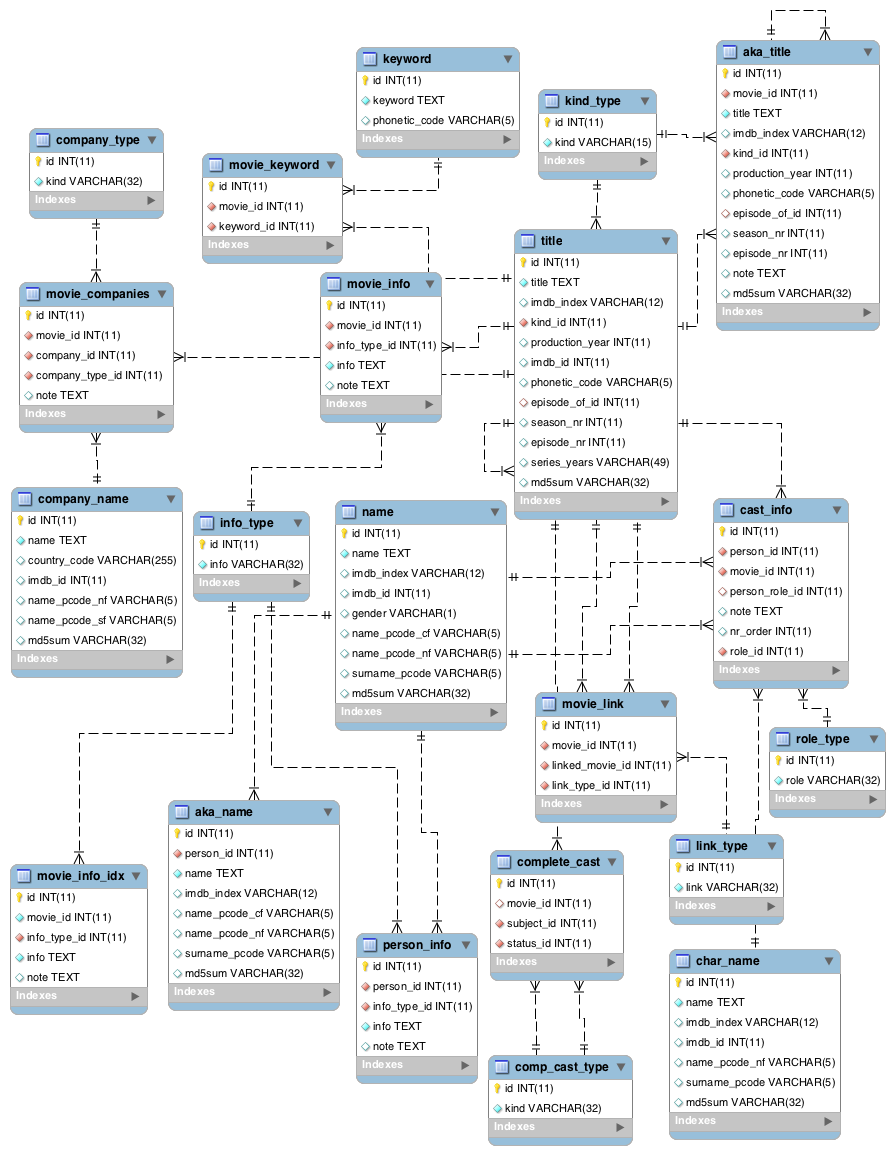
\includegraphics[width=3.5in]{ERgraph.png}
	\caption{IMDB Database Relational Schema}
	\label{fig:side:a}
\end{figure}

We tried several queries on the built database, such as finding the movie with the largest amount of budget or gross. The results are not always correct. For example, the values of budget are strings like "\pounds 998,852" or "\$102,437 (USA)" which makes us unable to find the movie with the largest amount of budget with simple SQL query. Besides, the database doesn't contain rating information of movies which is a crucial factor for our analysis. So in the next round, we tried to load the files directly into R.

\subsection{Parsing Data in R}

The downloaded original files were too large to effectively load in R. The computation time and complexity are also a big challenge that our computer cannot handle. So we decide to build a reasonable sample dataset. A python script which can make a unique http request and retrieve data sample randomly is used. As our classification and clustering are based on the genre of movies, there are many attributes that are useless for us, such as seriesID, season, Episode, and etc. We choose to drop these columns during data cleaning process. After processing, the movie dataframe contains 11142 rows of records and 31 attributes for each record.  There are 29 genres in total in our dataset as shown in Figure 2. Except for the genre of "Other", the most popular genres are "Romance", "Documentary", "Drama", "Comedy".

There is one crucial problem that will influence our analysis in the following parts is that we noticed there are many missing values in the data. Almost every rows have one or more N/A value in different attributes. It is not possible to delete rows with missing value since it results in deleting almost the whole data. It is also impossible to replace the missing value because the values are strings, stratagies in data cleaning dealing with missing values are not suitable for this case.


\begin{figure}
	\centering
	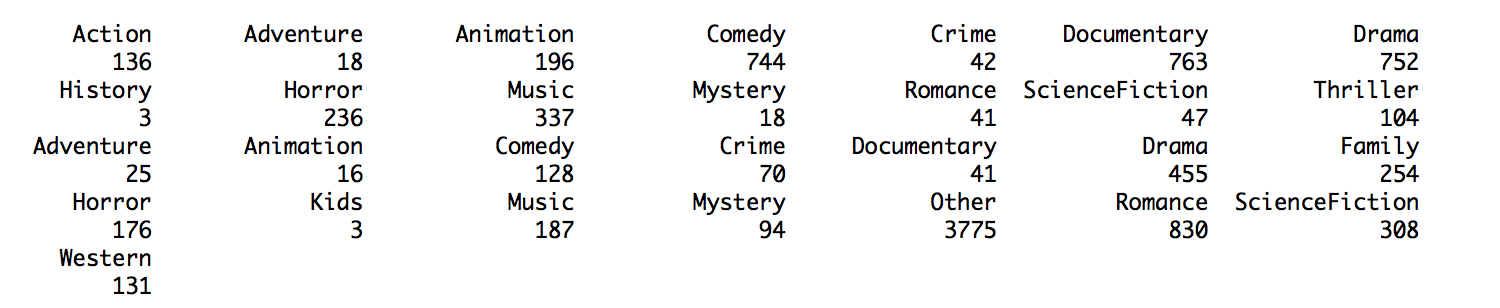
\includegraphics[width=3.5in]{genre_count}
	\caption{All Genre}
	\label{fig:side:a}
\end{figure}

\begin{figure}
	\centering
	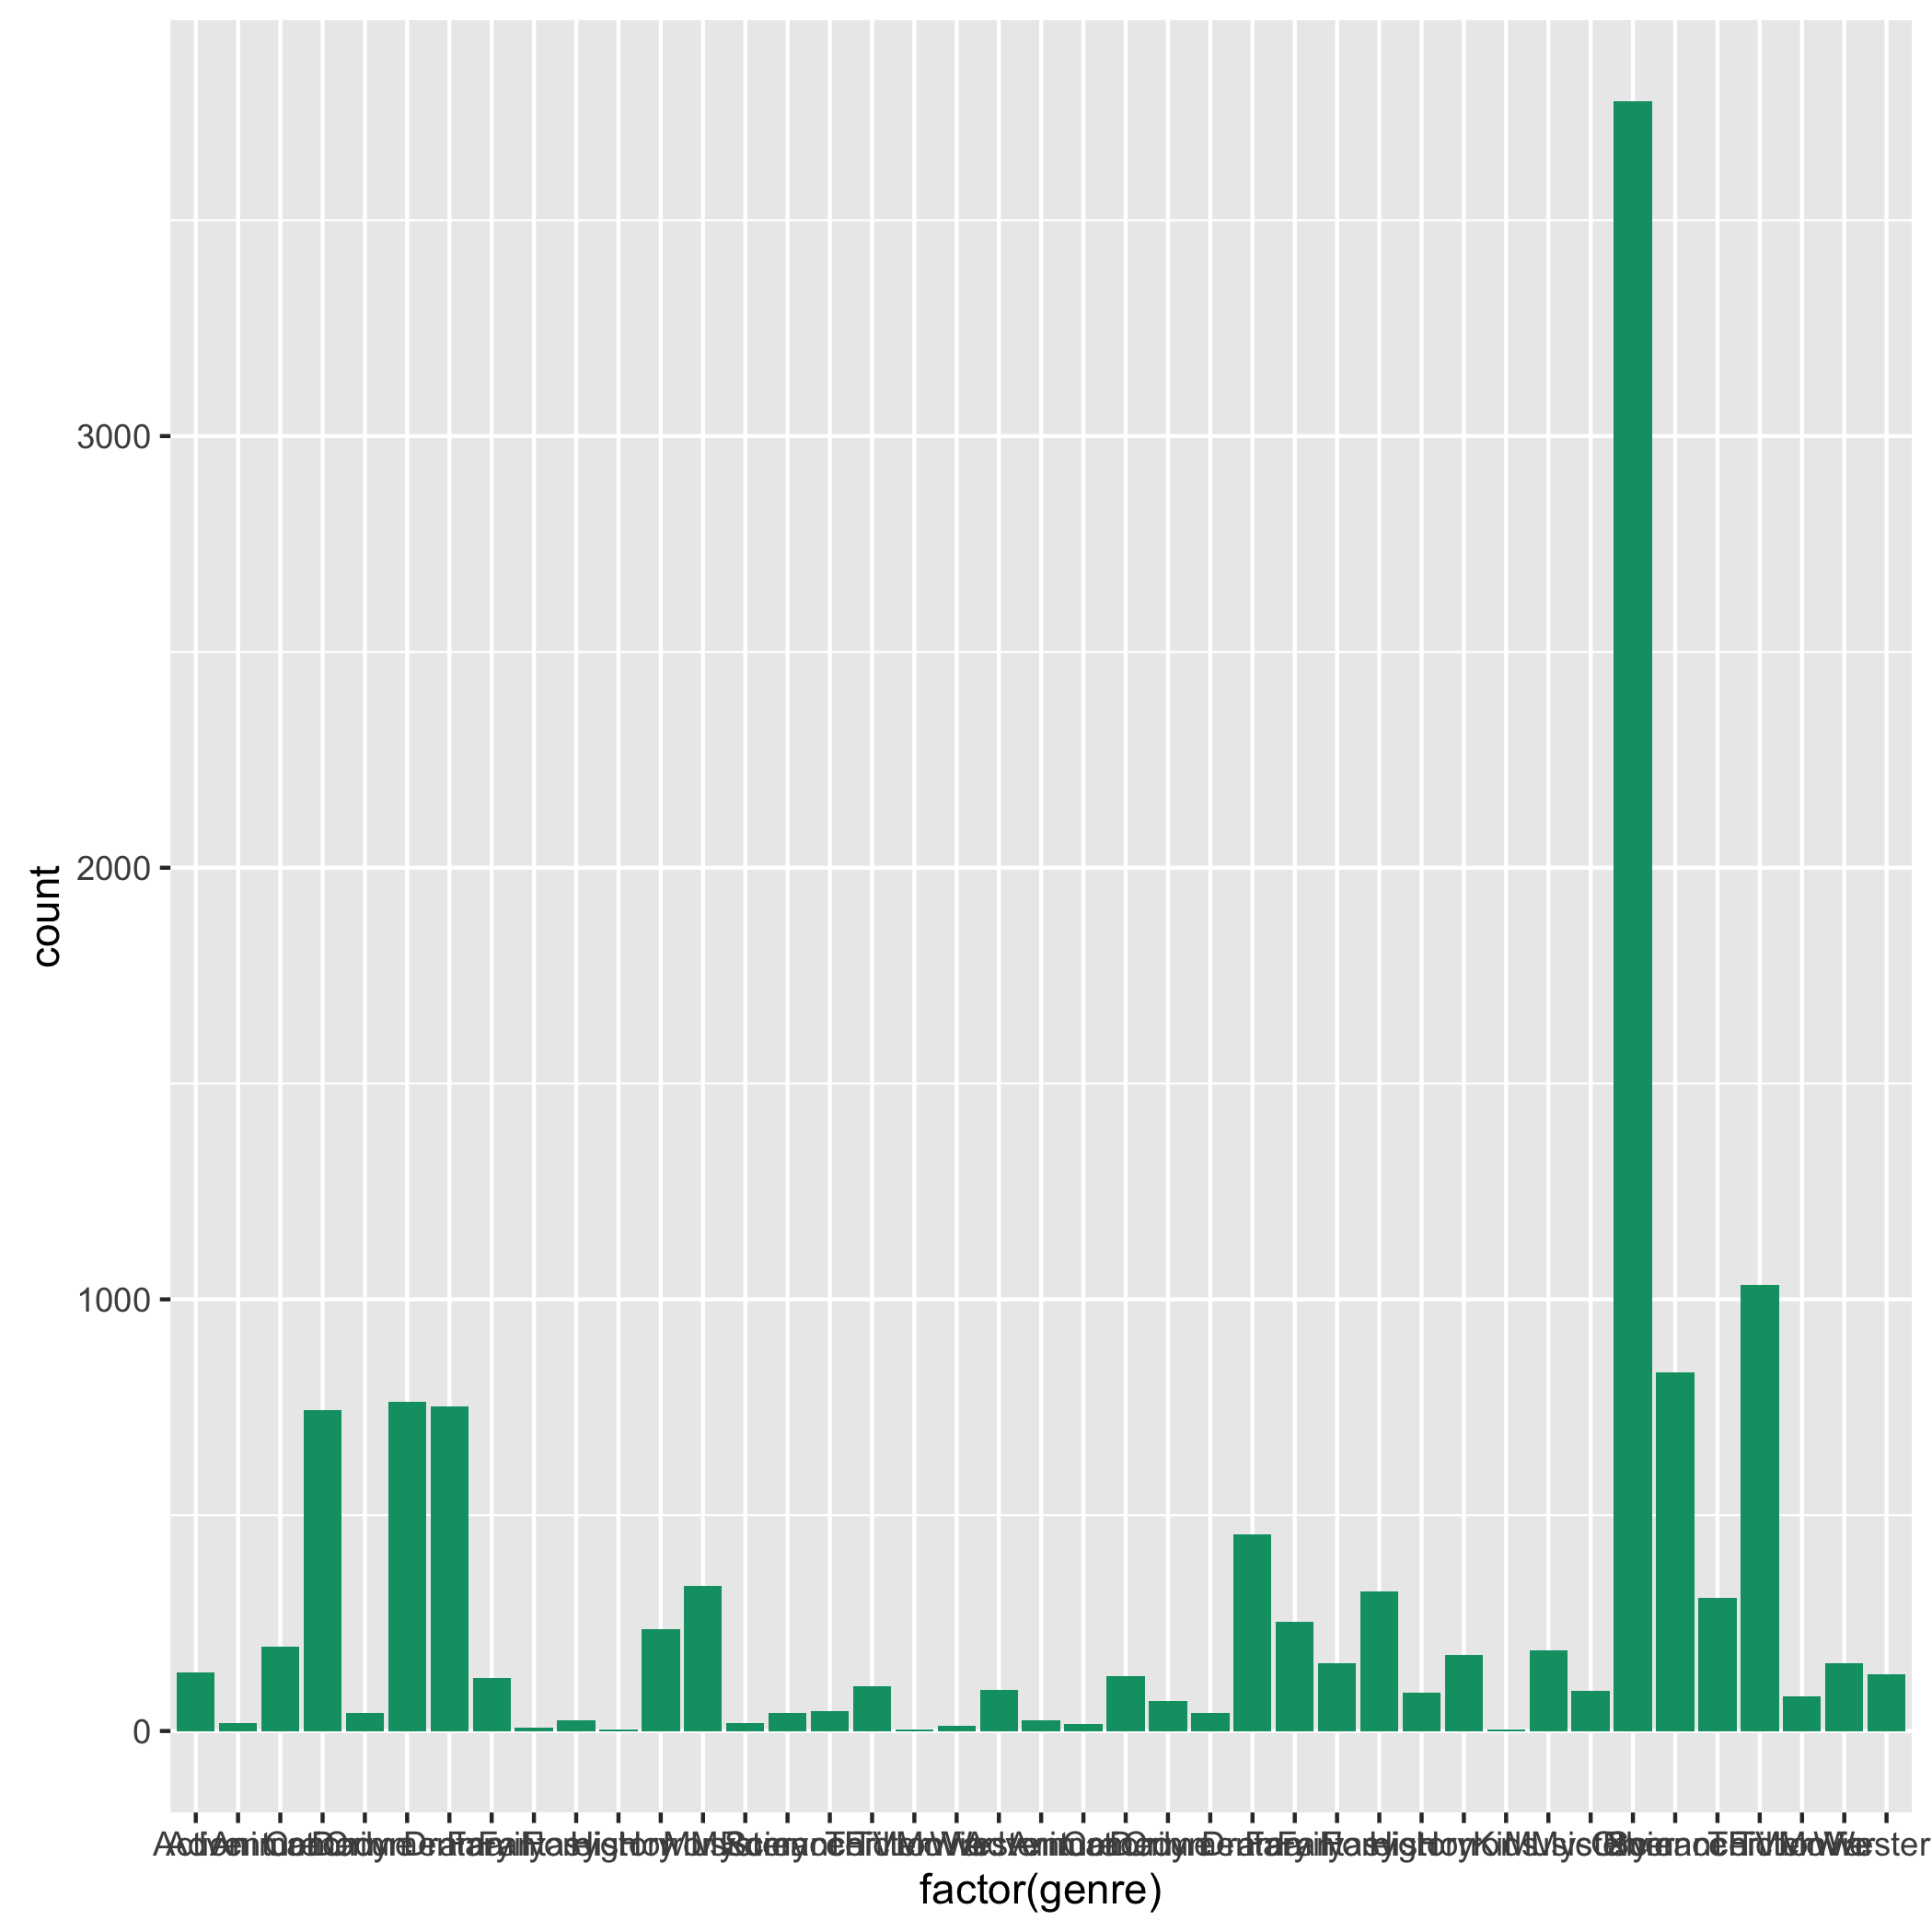
\includegraphics[width=3.5in]{genre_dis.png}
	\caption{Genre Distribution}
	\label{fig:side:a}
\end{figure}

We count the number of each genre in the sample set and plot the histogram as Figure 3. The rating range in IMDB is from 1 to 10. From Figure 4, we can see that more than 90\% of the movies have rating between 5 to 7.5. The maximum rating is 9.6 while the minimum rating is 1.

\begin{figure}
	\centering
	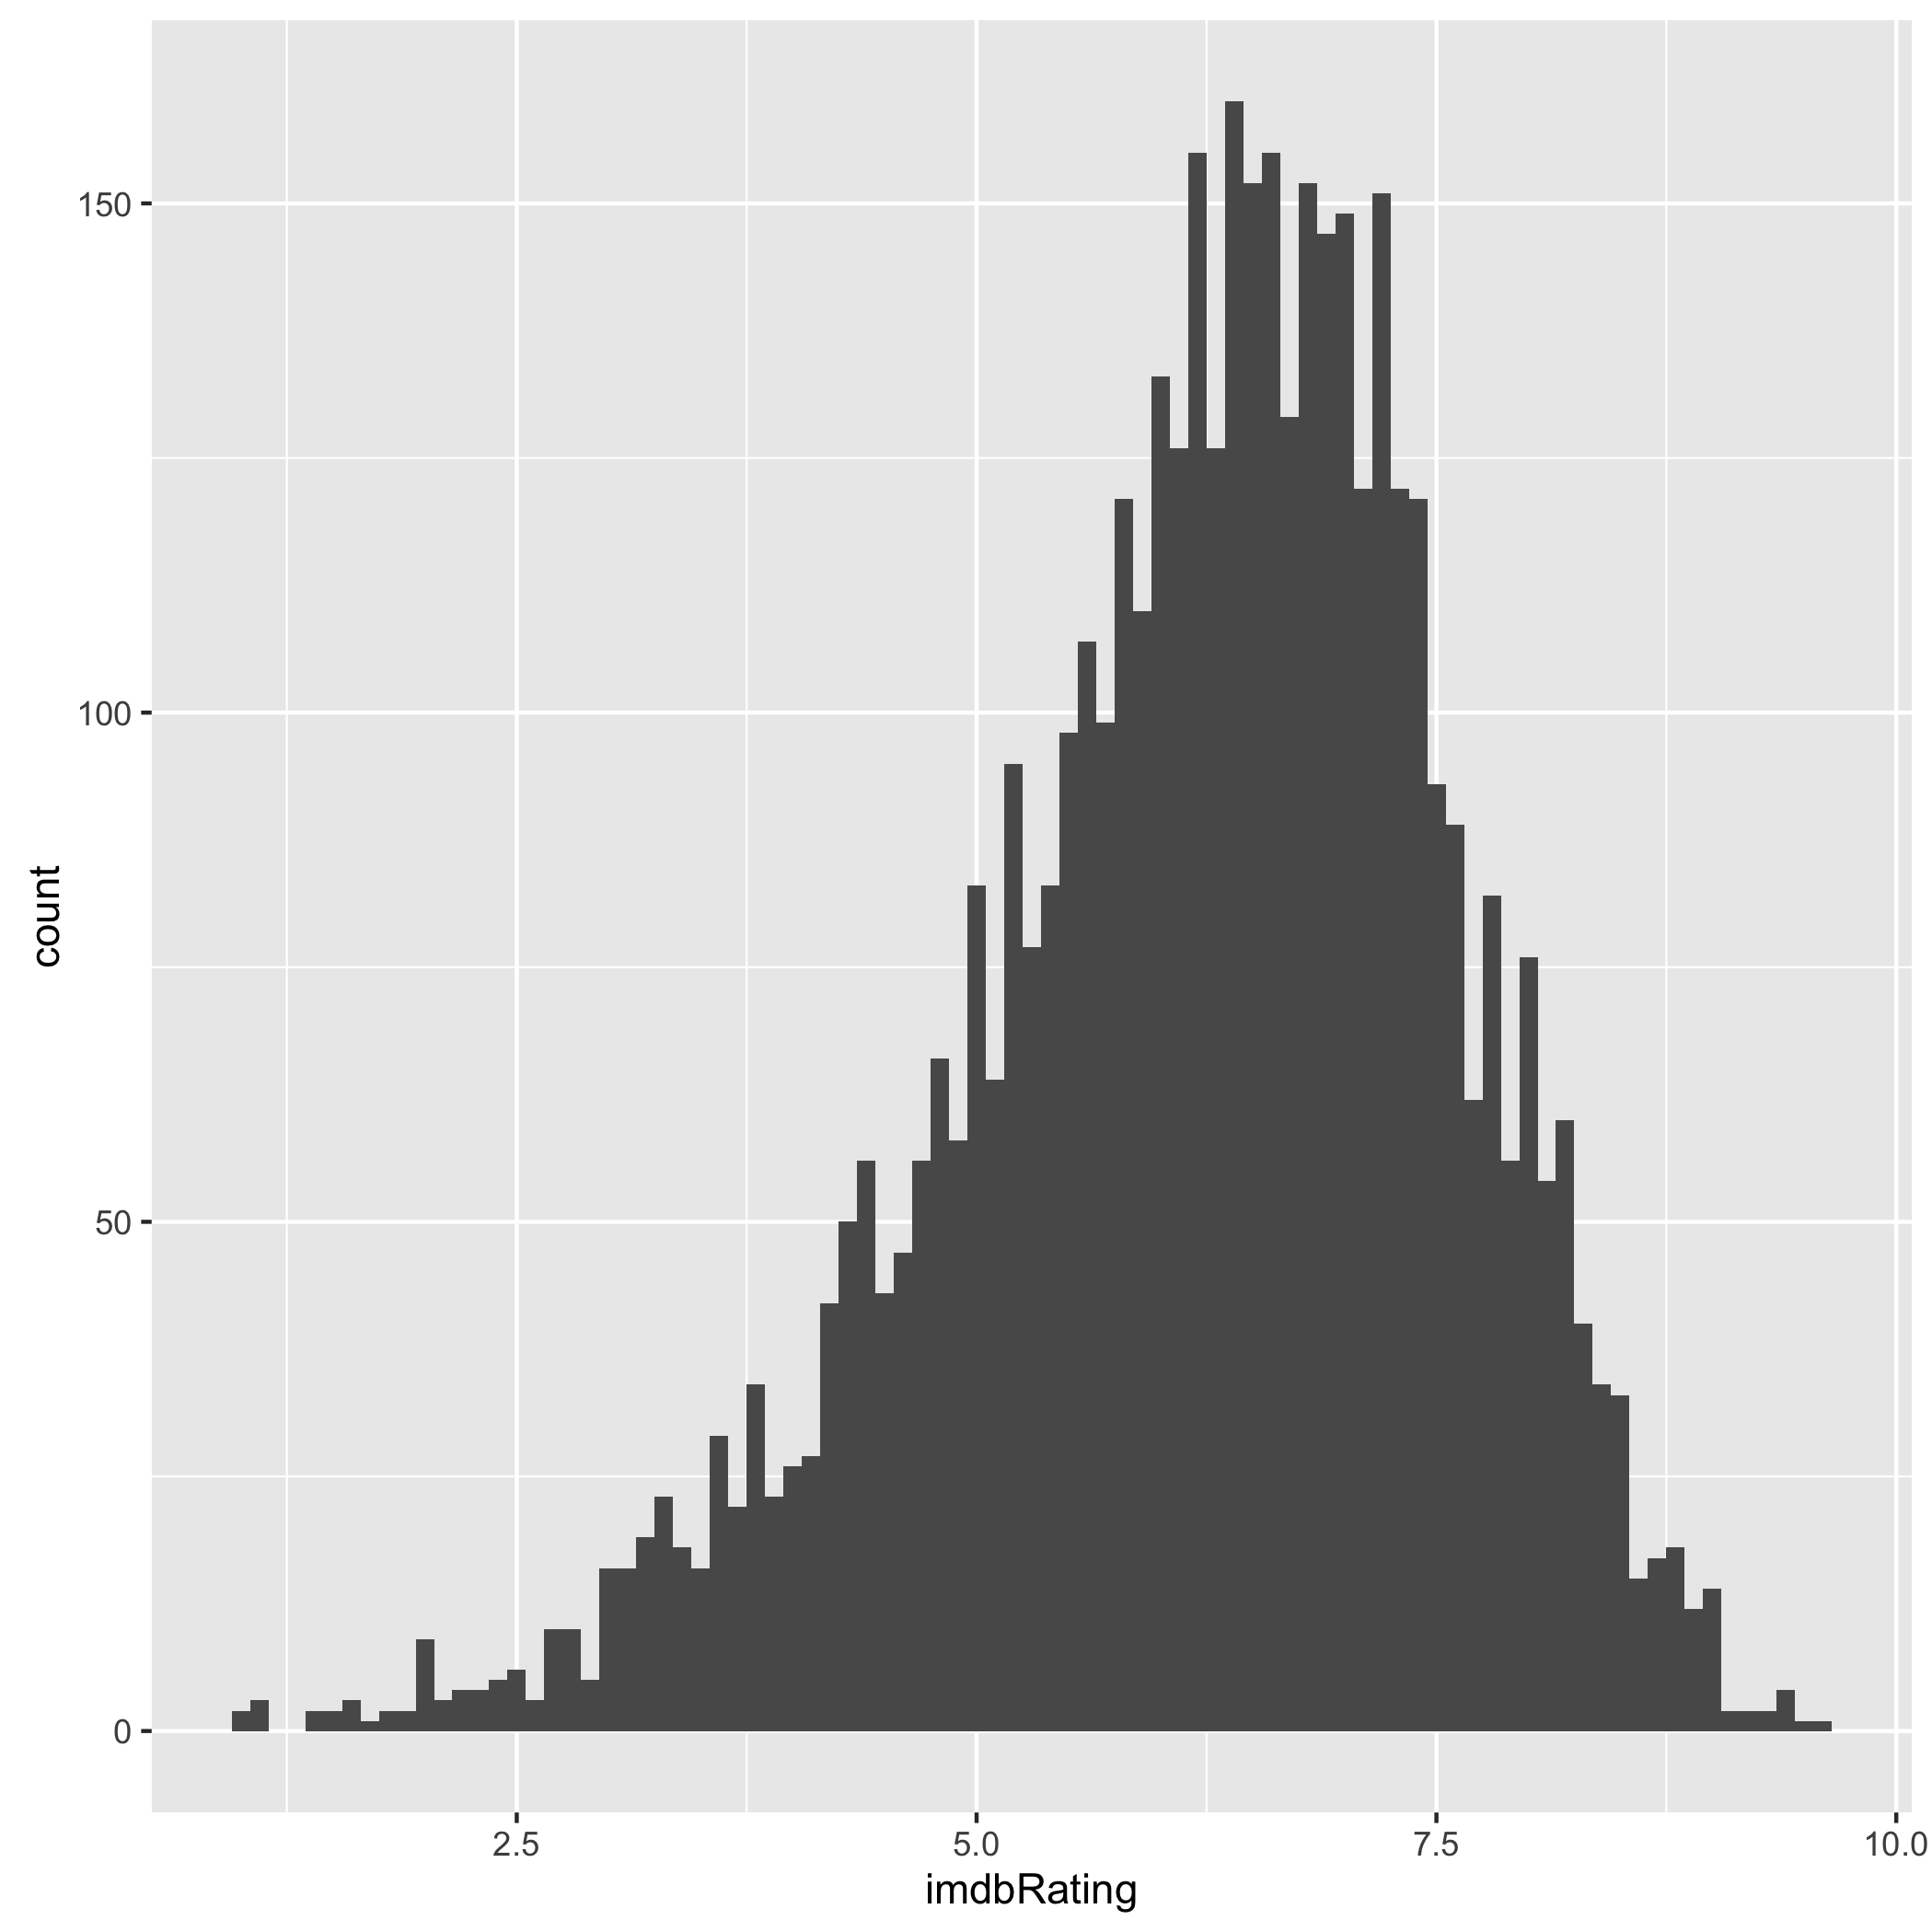
\includegraphics[width=3.5in]{rating_count.png}
	\caption{Rating Distribution in IMDB}
	\label{fig:side:a}
\end{figure}

Figure 5 shows the movie numbers in each year from 1891 to 2018. There is a clear and exponential increase in the number of movies with the increase of the year, especially during the latest 20 year. This is reasonable as it is consistant with reality which can be inferred to correspond to the growth of the movie industry over time.

\begin{figure}
	\centering
	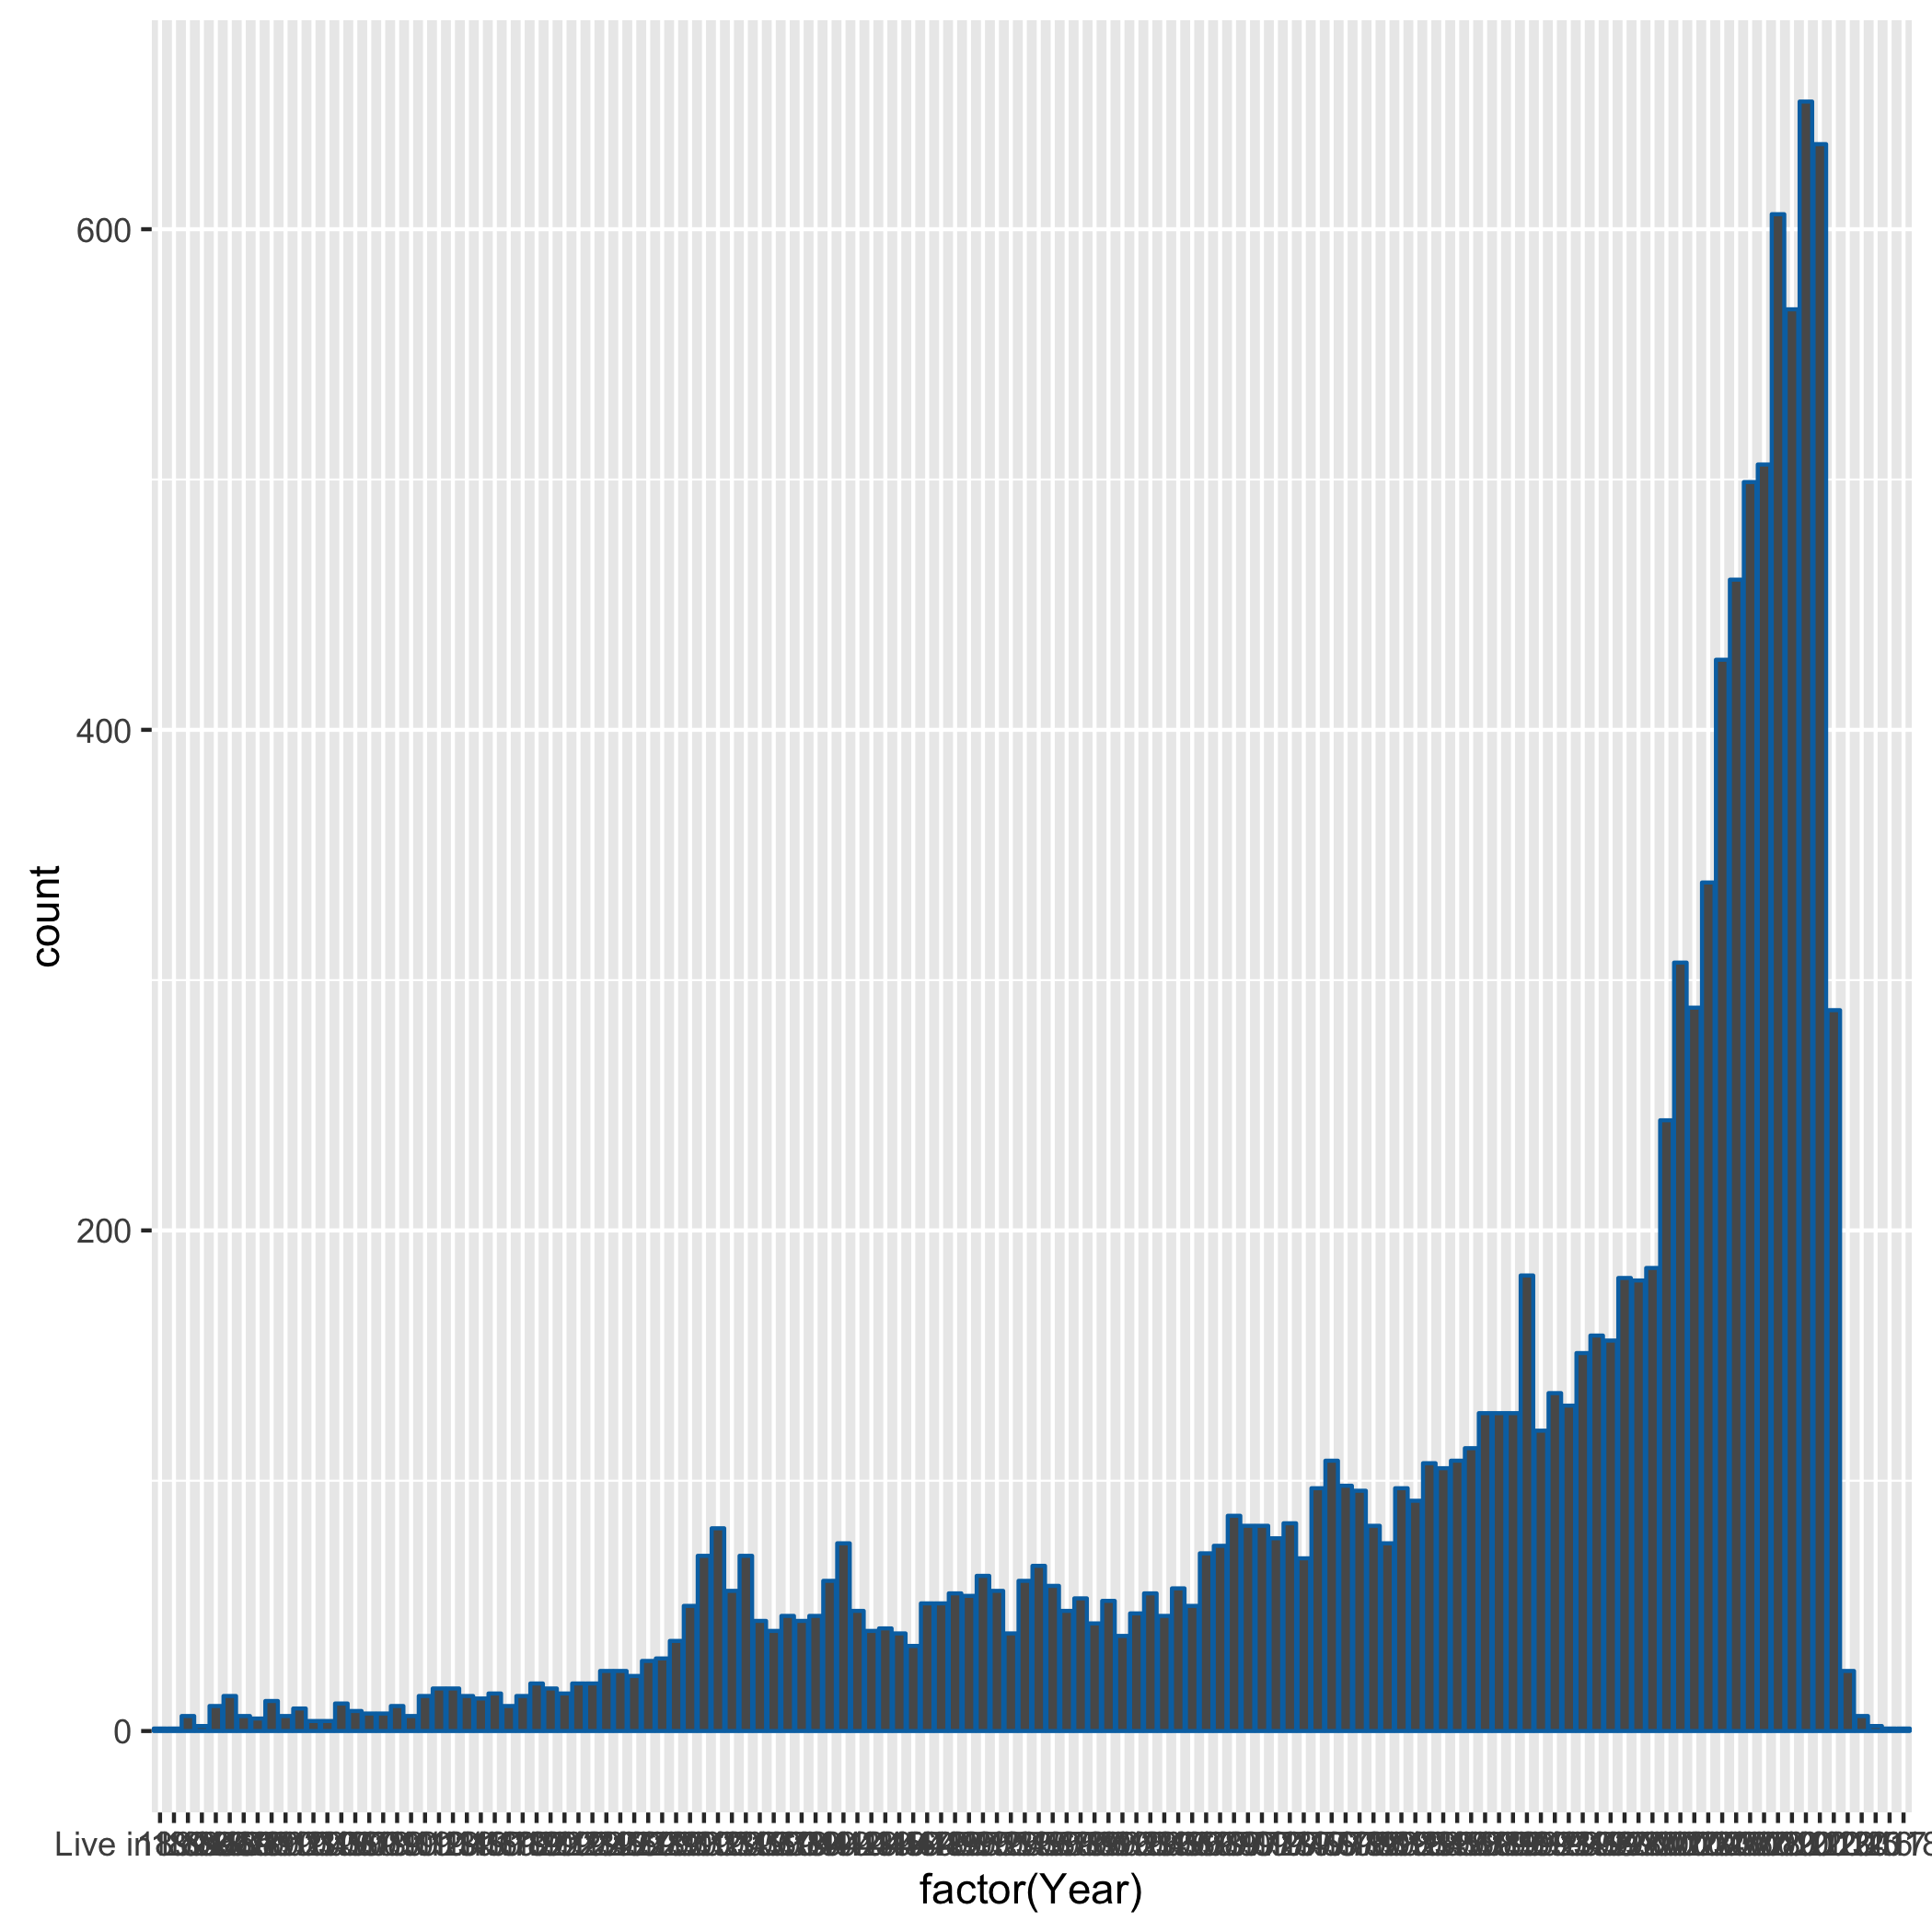
\includegraphics[width=3.5in]{year_count.png}
	\caption{Movie count by Year}
	\label{fig:side:a}
\end{figure}

The IMDB provided a ranking list of top250 movies. The ranking is based on both the rating and voting counts of movies. So we plot a figure of voting numbers against the ratings. The scatter plot is shown in Figure 6. We can see that the distribution is similar to the rating distribution in Figure 4.
\begin{figure}
	\centering
	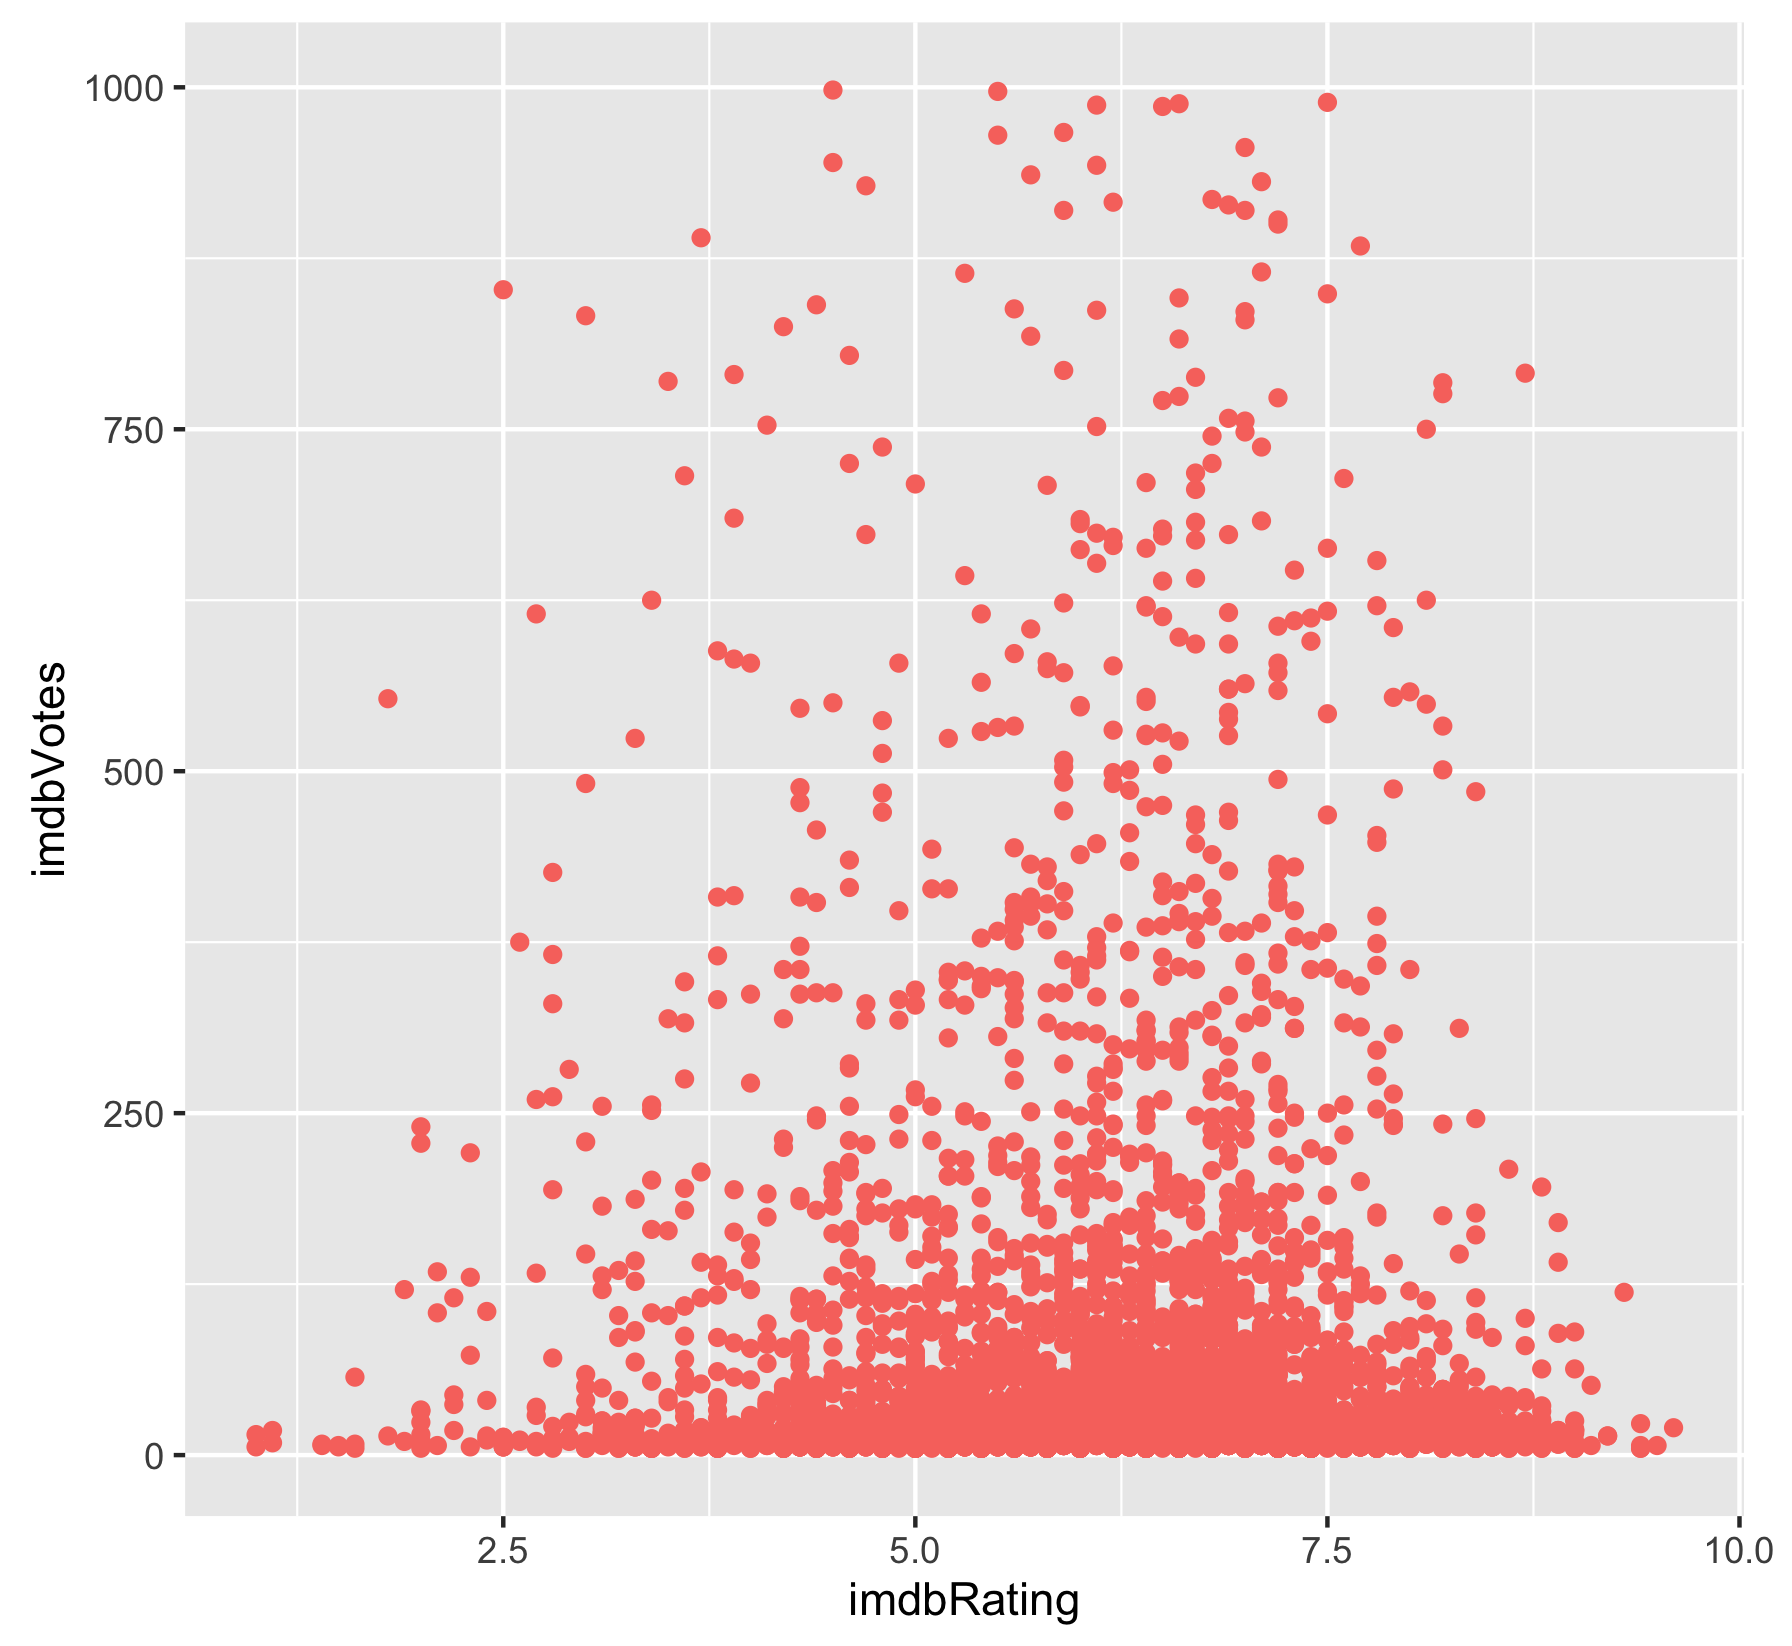
\includegraphics[width=3.2in]{vote.png}
	\caption{Vote Count by Rating}
	\label{fig:side:a}
\end{figure}

\section{Methodologys}
\subsection{Association Rules}

Association rules are information gathered from datasets. Data mining are interested in discovering relations between attributes that always occur together for prediction and recommendation. 

Formulation of the Association Rules Mining problem\cite{Michael}:
Given a dataset of $n$ samples $S = \{s_1, s_2, ......, s_n\}$, where each sample has $k$ items $s_i = \{I_{i1}, ......, I_{ik}\}$, the total possible items $I = \{I_1, ......, I_m\}(k\leq m)$.  An association rule is an implication in the form of $x\Rightarrow y$, where $x$, $y$ are subsets of I and disjoint, also known as itemsets. Following are some definition of concepts in the Association Rules Mining.

\textit{Support.} The support of an itemset $x$ with respect to a dataset is the proportion of samples in which $x$ occurs in the dataset
\begin{equation*}
support(x) = \frac{the number of samples contain x}{the number of total samples}.
\end{equation*}
  
The support of an association rule $x\Rightarrow y$ with respect to a dataset is the proportion of samples in which itemsets $x$ and $y$ occur together in the dataset
\begin{equation*}
support(x\Rightarrow y) = \frac{the number if samples contain x and y}{the number of total samples}.
\end{equation*}


\textit{Confidence.} The confidence of an association rule $x\Rightarrow y$ with respect to a dataset is the ratio of number of samples in which itemsets $x$ and $y$ occur together to the number of samples in which as long as itemset $x$ occurs in the dataset 
\begin{equation*}
confidence(x\Rightarrow y) = \frac{the number of samples contain x and y}{the number of samples contain x}.
\end{equation*}

The confidence of $x\Rightarrow y$ can also be presented by the ratio of the support of $x\Rightarrow y$ to the support of itemset $x$
\begin{equation*}
confidence(x\Rightarrow y) = \frac{support(x\Rightarrow y)}{support(x)}.
\end{equation*}


\textit{Lift.} The lift of an association rule $x\Rightarrow y$ with respect to a dataset is defined as the ratio of  the support of $x\Rightarrow y$ to the product of the support of itemset $x$ and the support of 
itemset $y$
\begin{equation*}
lift(x\Rightarrow y) = \frac{support(x\Rightarrow y)}{support(x)\cdot support(y)}.
\end{equation*}


As many association rules are inadequate and useless due to some items occur together by 
chance, it is necessary to set thresholds for support and confidence respectively for reducing such association rules. 

In conclusion, the Association Rule Mining problem is to find out those association rules of which support and confidence above given support and confidence thresholds. 

\subsection{Classification}
As we have got the main genre for every movie sample after preprocessing the original dataset, we will carry on a genre prediction using some classification methods. Classification is a supervised approach in the field of data mining, and it discovers a knowledge pattern from a training set of data of which the class membership is already labeled, then use this pattern to identify every entry of a new set of data, call testing set, belong to which class. There are a lot of specific methods of classification, such as K-Nearest Neighbours(K-NN), Support Vector Machine(SVM), Naive Bayes classifier, Decision Tree, Neural Network.
In this project, these classification algorithms as following are used to predict the genre of a movie sample:  K-Nearest Neighbours, Naive Bayes classifier, C4.5, RIPPER, Oblique Tree. It is worthy to notice that the last three methods belong to Decision Tree. 
\subsubsection{K-Nearest Neighbours}
K-NN is a similarity based classifier, the label of a testing entry is associated with the label of its neighbours. When given a testing set of data, first calculate each entry’s K nearest neighbours in the training set defined by the closeness between them, usually on the basis of a specific distance function or other metrics. After generating K nearest neighbours, the algorithm finds out their labels and take a vote. In another word, an entry is assigned to the most common class among its K nearest neighbours. 
In practice, the value of K should be chosen not too large or too small\cite{Everitt}. Though large value of K reduce the effect of noise, it makes less distinct boundaries between classes and leads to a underfitting problem. In the contrast, small value of K will cause overfitting. Therefore, we choose a proper K under the guideline that it should be odd and  where n is the number of samples.

\subsubsection{Naive Bayes classifier}
Naive Bayes classifier is a probabilistic approach based on Bayes theorem and make a strong assumption that the value of every attribute of a sample is independent with each other\cite{Narasimha}. Bayes Formula is as follows: 
\begin{equation}
P(c_i|s) = \frac{P(s|c_i) \cdot P(c_i)}{P(s)}
\end{equation}
$c_i$ is class $i$ and $s$ is a sample
where $P(c_i|s)$ is called posterior, $P(s|c_i)$ is called likelyhood, $P(c_i)$ is called prior, $P(s)$ is called evidence.

Bayes decision rule:

if $P(c_1|s) > P(c_2|s)$, $s$ belongs to class 1;

else if $P(c_1|s) < P(c_2|s)$, $s$ belongs to class 2. 

Naive Bayes classifier assumes a sample has d discrete­valued attributes, $s = (a_1, ......, a_d)$. Therefore, 
\begin{equation*}
P(s|c_i) = P(a_1, ......, a_d|c_i) = \prod^d_1P(a_j|c_i).
\end{equation*}


We can learn likelihood and prior from the training dataset, as $P(a_j|c_i)$ can be evaluated by calculating the fraction of samples in class i share the same feature values, prior $P(c_i)$ is equals to number of samples in class i / number of all samples, moreover, evidence $P(s)$ is identical for all samples. Thus, it is possible to assign each new sample a class label based
on the learning of training dataset, 
\begin{equation*}
P(c_i|s^new) = \frac{\prod^d_1 P(a_j|c_i) \cdot P(c_i)}{P(s)}.
\end{equation*}


\subsubsection{C4.5}
Iterative Dischotomiser 3 (ID3), which is used to generate a decision tree from the training dataset. This algorithm regards the training dataset as a root node at the beginning. During each iteration, it uses every attribute to split the dataset and calculates the Entropy and Information Gain of the selected attribute, then choose the attribute which leads to a largest Information Gain as the partition attribute and generate subsets of the original dataset. Recursion will be applied to each subset considering only non­partition attribute. The recursion will be stopped in some cases: in the subset, every sample belongs to the same class, then the node is assigned with the class label and becomes a leaf node; there are no more non­partition attribute, then the node is assigned with the most common class label and becomes a leaf node; there no samples correspond to the condition, then the node is assigned with the most common class label in its parent node and becomes a leaf node\cite{Quinlan}. 

C4.5 makes some improvements to ID3. First, it handles both continuous and discrete attributes with a threshold metric. Then, once a decision tree is created, it is able to replace branches not helping with leaf nodes, which is known as pruning. Finally, it can deal with missing attribute values in training dataset by ignoring them in the process of calculating Entropy and Information Gain, which is also a main reason for us to use C4.5 instead of ID3 as the dataset has some missing values of attributes.

\subsection{Clustering}
Compared with classification, clustering is an unsupervised approach of data mining. Thus, we create a new dataset without attribute “genre”, and there is no need to divide the dataset into training and testing dataset. However, after applying clustering algorithm on the dataset, we will use the attribute “genre” in the original dataset to measure how good the performance of the method is.

As there are both numeric and nominal values of attributes in the dataset, we will not use traditional approaches, such as K­Means, Fuzzy C­Means and DBSCAN, which are based on distance metric. Instead, we choose Robust Clustering using links (ROCK) to cluster the dataset into clusters within the number of genres.

ROCK evaluates the similarity between samples with the number of shared neighbours rather than distance, then a hierarchical clustering scheme is used to cluster the dataset. Thus, it can handle nominal attribute values with this special link and perform better than other traditional algorithms\cite{Guha}.

\subsection{Collaborative Filtering}

Collaborative filtering filters information by using the recommendations of other people. It is based on the idea that people who agreed in their evaluation of certain items in the past are likely to agree again in the future. A person who wants to see a movie, might ask for recommendations from friends. The recommendations of some friends who have similar interests are trusted more than recommendations from others. This information is used in the decision on which movie to see. The above is the basic idea of our implementation is this part.

Typically, collaborative filtering adopts the neighborhood-based technique. There are two kinds of approach: user-based and item-based.

\textit{User-based collaborative filtering}, also know as \textit{k-NN collaborative},was the first of the automated CF methods. It find other users whose past rating behavior is similar to that of current user and
use their ratings on that item to predict what the current user will like. 

\textit{Item-based Collaborative Filtering} is similar to User-based CF, it uses similarity between the rating patterns of items. If two items tend to have the same users like and dislike them,then they are similar and users are expected to have similar preferences for similar items.
\subsubsection{Computing Predictions}
To compute predictions or recommendations for a user u, user-user CF firstly needs to determine the number N of neighbors will be used to generate the result. Then computing the weighted average of the chosen neighboring users' rating i by using similarity as weights\cite{survey}. The formula is given as below:

\begin{equation}
p_{u,i} ={\bar r_{u}}  + \frac
{\sum\nolimits_{u' \in N} s(u,u')(r_{u',i} - {\bar r_{u'}})} 
{\sum\nolimits_{u' \in N} |s(u,u')|}
\end{equation}

In order to eliminate the differences in users's use of the rating scale, subtracting the user's mean rating ${\bar r_{u'}}$ to compensate is necessary.   The parameter $p_{u,i}$ is predicated rating on item i for user $u$.  ${\bar r_{u'}}$ is average rating on all items rated by user $u$.The parameter $r_{u',i}$ indicates the rating of user $u'$ on item i.$s(u,u')$ is similarity between user u and $u'$. N is the number of neighbors chosen for user $u$.  

\subsubsection{Measure of Similarity}
An critical parameter used to calculate predications is similarity function. One of the most common and typically measurements is the cosine similarity. 

In Cosine Similarity model, users are represented as $|\textit{I}|$-dimensional vectors of rating on $|\textit{I}|$ items. Similarity is measured by the cosine distance between two rating vectors. The formula is given below indicating how to calculate the Cosine Similarity between user $u$ and $v$ \cite{Herlocker}. 
\begin{equation}
s(u,v) = \frac{\sum\nolimits_{i} r_{u,i}r_{v,i}}{\sqrt{\sum\nolimits_{i} {r^{2}_{u,i}}} \sqrt{\sum\nolimits_{i} {r^{2}_{v,i}}}} 
\end{equation}

$r_u$ is rating vector of user $u$.

\subsubsection{Evaluation Metrics}
Our goal is to predict the rating a user would give to a restaurant. We predict the rating that user has not rated in the training dataset, but the true rating is stored in the test dataset. We use the root-mean-square error and mean-absolute error for evaluation.
\begin{equation}
\ RMSE = \sqrt{\frac{\sum{\left(r'_{u,i} - r_{u,i}\right)}^2}{N}}
\end{equation}
\begin{equation}
\ MAE = \sqrt{\frac{\sum{\left|r'_{u,i} - r_{u,i}\right|}}{N}}
\end{equation}

Here $r'_{u,i}$ is the predicted rating from user $u$ on item $i$ and $r_{u,i}$ is the true rating; $N$ is the size of test dataset. 

Another evaluation method is precision-recall: precision tells us how good the predictions are. In other words, how many were a hit; recall tells us how many of the hits were accounted for, or the coverage of the desirable outcome.
\begin{equation}
\begin{split}
& precision = \\
& \frac{\left|\{relevant documents\}\bigcap \{retrieved documents\}\right|}{\left|\{retrieved documents\}\right|}
\end{split}
\end{equation}

\begin{equation}
\begin{split}
& recall = \\
&\frac{\left|\{relevant documents\}\bigcap \{retrieved documents\}\right|}{\left|\{retrieved documents\}\right|}
\end{split}
\end{equation}


\section{Experimental Evaluation }
\subsection{Classification}
After preprocessing the original dataset by deleting non­movie, approximately two­thirds samples were dropped.Then, we ignore the useless attributes for data mining and divide the original dataset into two new dataset: training dataset with attribute “genre” and testing dataset without attribute “genre”. In addition, because there are a several hundred of genre in the original dataset, we choose 29 genres having sufficient support samples. Furthermore, many samples have more than one genre, in order to evaluate the performance of methods, we only take into account a main genre for these samples.These new datasets provide abundant information for genre prediction. We apply classification algorithms on training dataset to generate a learning model and then use it on testing dataset to predict the genres of movie samples.
\subsubsection{K­Nearest Neighbours}
It is already mentioned in section 5 the reason for choosing a proper value of k. However, even if we choose the best value for parameter k, due to many samples contain null values and every sample has both nonminal and numeric attribute values, the performance of K­-NN is poor as it is a distance based approach. The accuracy of K-NN is 5.73\%.

Accuracy : 0.0573

95\% CI : (0.0324, 0.0927)

No Information Rate : 0.2366

P-­Value [Acc $>$ NIR] : 1

Kappa : -0.0534

Mcnemar's Test P­-Value : NA 

\subsubsection{C4.5}
Although the classification performance of C4.5 is not good enough, it is still better than K-NN. One reason for this is that C4.5, one of Decision Tree algorithm, has the ability of dealing with nonminal attribute values, which K-NN is lack of. The accuracy of C4.5 is 17.14\%.

Accuracy : 0.1714

95\% CI : (0.1581, 0.1854)

No Information Rate : 0.2686

P-­Value [Acc $>$ NIR] : 1 

Kappa : 1e­08

Mcnemar's Test P-­Value : NA

\subsubsection{Naive Bayes classifier}
This classification approach shows the best performance of the three methods as it has the highest accuracy. This is likely due to that each attribute is considered as independent and make a contribute to the probability of the sample belonging to a specific class. The accuary of NB is 34.29\%.

Accuracy : 0.3429

95\% CI : (0.3259, 0.3602)

No Information Rate : 0.2686 

P­-Value [Acc $>$ NIR] : $<$ 2.2e-16

Kappa : 0.2377

Mcnemar's Test P­-Value : NA

The classification accuracy of the three methods is compared in table1.
\begin{table}
	\caption{Comparison of Different classification methods}

		\begin{tabular}{cccc}
			\hline
			\rule{0pt}{12pt}Methods  & \rule{0pt}{12pt}Accuracy  & \rule{0pt}{12pt}95\% CI   &\rule{0pt}{12pt} No Information Rate\\
			\hline\rule{0pt}{12pt}
			K-Nearest Neighbours    &   0.0573 & \ (0.0324, 0.0927)	 & \ 0.2366 \\
			C4.5   &  0.1714  & \ 	 (0.1581, 0.1854) & \ 0.2686 \\
		   Naive Bayes classifiere   &   0.3429 & \ (0.3259, 0.3602) & \ 0.2686 \\
			\hline
		\end{tabular}

\end{table}


\subsection{Clustering}
We perform a similar preprocess on the original dataset as the way we do for classification. The different is that after eliminating non-movie samples, useless attributes and choosing the main genres of samples, we keep a copy but delete the attribute “genre” for clustering, and use the one with attribute “genre“ to measure the performance.

ROCK clustering algorithm can deal with nonminal attribute values, which is a significant strength from other traditional clustering algorithm. First, the link value between each pair of samples are computed using the number of shared neighbours between them to reflect the dissimilarities. Then, with the dissimilarity and a objective function which is to maximize the shared neighbours, an agglomerative hierarchical clustering is applied on the dataset. Finally, those samples have not assigned cluster labels will be put in the clusters found.

After applying ROCK clustering algorithm on the dataset, it is divided into 723 clusters. This number is pretty larger than the number of genres that we choose, 29. A reason for this is that maybe some movie samples with a hybrid genre have been considered in distinct clusters. It is reasonable and consistent with dataset preprocessing, where we choose the main genre of each this kind of sample. Another reason is that though some movie samples share the same genre, their other attributes are not such similar that the algorithm can not differentiate them into the same cluster. As clustering is an unsupervised approach, it is easy to understand that its limitations are more than classification.

\subsection{Association Rules Mining}
The Brute Force method of mining association rules is that list all possible rules on the basis of subset of itemset I, and select those whose support and confidence are larger than given thresholds. However, since our dataset has a large amount of samples, it is not practical to apply this method. In addition, two observations can be discovered from the definition of association rules: those rules with large support consist of itemsets with large support, which is also known as large itemsets; any subset of a large itemset is also large, in contrast, if a large itemset contains a non-large subset, it is not large either.

As above indicates, we choose Apriori Algorithm\cite{Borgelt} to implement association rules mining.In the first pass, it examines every item in the itemset I, determine which part are large itemsets of size 1, and prunes those non-large itemsets. Then, it permutates 1-size large itemsets to 2-size itemsets which are candidate large itemsets. Again, supports and confidences are calculated and compared with the specified thresholds to decide whether those candidates are large itemsets and prune non-large ones. It makes a recursion on the candidates until there is no more candidate.

Owing to that in the original dataset, there are too many attributes and we are not interested in the relationships between some attributes, we produce two new datasets. One is comprised of leading roles, their two most significant supporting roles and three high-ranking crews got from each movie they participated in. Another includes crews and movies’ genres.

After performing Apriori Algorithm on our new dataset and deleting those redundant association rules, we set thresholds for support and confidence as 0.0002 and 0.9, then select top 10 and 10 rules respectively. The rules are shown in the table 2 and table 3.

\begin{table}[!hbp]
	\caption{The usual lists of actors}
	\begin{center}
	
	\begin{tabular}{|c||c|}
		\hline
		antecedent & consequent \\
		\hline
		\{supporting role1 = Divine, & \{leading role = \\
		 supporting role2 = David Lochary\}  &  Mary Vivian Pearce\}  \\
		 \hline
		 \{supporting role1 = Divine, & \{leading role = \\
		 supporting role2 = Mary Vivian Pearce\}  &  David Lochary\}  \\
		 \hline
		 \{supporting role1 = Divine, & \{leading role = \\
		 supporting role2 = David Lochary,  &  Mary Vivian Pearce\}  \\
		 crew = John Waters\} &   \\
		  \hline
		  \{supporting role1 = Divine, & \{leading role = \\
		  supporting role2 = Mary Vivian Pearce,  &  David Lochary\}  \\
		  crew = John Waters\} &   \\
		\hline
		\{supporting role1 = David Lochary\} & \{leading role = Divine\}\\
		\hline
		\{supporting role1 = David Lochary\} & \{leading role = \\
		 &  Mary Vivian Pearce\}  \\
		 \hline
		 \{supporting role1 = David Lochary, & \{leading role = \\
		 supporting role2 = Mary Vivian Pearce\}  &  Divine\}  \\
		 \hline
		 \{supporting role = David Lochar, & \{leading role = \\
		 crew = John Waters\}  &  Divine\}  \\
		 \hline
		 \{supporting role1 = David Lochary, & \{leading role = \\
		 supporting role2 = Mary Vivian Pearce,  &  Divine\}  \\
		 crew = John Waters\} &   \\
		 \hline
		  \{supporting role1 = Joe Pennyr, & \{leading role = \\
		  supporting role2 = William R. Moses\}  &  Lea Thompson\}  \\
		  \hline
		  
	\end{tabular}
	\end{center}
\end{table}

We regard leading roles as primary key in this new dataset, and search the original dataset with every leading role to find out the movies they take part in, then extract the supporting roles and crews in the movies, count the number and make a ranking to choose the top two supporting roles and three crews for each leading role as his attribute in the dataset. We produce this dataset for the reason that it is typical that some actors always cooperate together in the  movies of a specified genre.

The Apriori algorithm generates thousands of rules and we choose 10 samples of rules to analyse. However, these 10 rules are highly related with the filmmaker John Waters and his co-workers Divine, David Lochary, Mary Vivian Pearce. It can be deduced that John Waters always make low-budget movies as himself play different roles in the same movie such as writer, director, producer and his actors are only several ones.

\begin{table}[!hbp]
	\caption{The crews and genres}
	\begin{center}	
		\begin{tabular}{|c||c|}
				\hline
				antecedent & consequent \\
				\hline
				\{crew = Walt Disney\} & \{genre = Animation\} \\
				\hline
				\{crew = Jules White\} & \{genre = Comedy\} \\
				\hline
				\{actor = Curly Howard\} & \{genre = Comedy\} \\
				\hline
				\{actor = Mel Blanc\} & \{genre = Family\} \\
				\hline
				\{actor = Vijayakanth\} & \{genre = Drama\} \\
				\hline
				\{crew = Ilayaraja\} & \{genre = Drama\} \\
				\hline
				\{crew = Robby D.\} & \{genre Other\} \\
				\hline
				\{crew = Dave Fleischer\} & \{genre = Other\} \\
				\hline
				\{crew = Mel Blanc\} & \{genre = Other\} \\
				\hline
				\{genre = Animation\} & \{actor = Clarence Nash\} \\
				\hline
			
		\end{tabular}
	\end{center}
\end{table}

For this new dataset, we discover each movie’s genre and the actors and crews participating in, since some actors almost exclusively show in several genres of movie throughout their careers and some directors focus on only one specified genre in decades. And the above rules have proved our assumption. For example, Walt Disney was an American entrepreneur, animator, voice actor and film producer, who co-founded The Walt Disney Company with his brother. Thus, almost every film he played a role in belongs to animation. In addition, in the second rule shown above that if a movie belongs to animation, Clarence Nash always shows. It is a little absolute but not wrong. Clarence Nash was an American voice actor, best known as the Disney cartoon character Donald Duck as he provided the distinctive voice for nearly fifty years. Moverover, he also provided Tom in Tom and Jerry with the voice, which is a famous and popular cartoon.

\subsection{Rating Prediction}
\subsubsection{Visualizing Data}
Data for this part is from the MovieLens dataset which is a rich resource for recommendation. We firstly visualize the data by ploting several histograms. Figure 7 is the rating distribution of the raw data. The rating range is from 1 star to 5 stars. Then we use a z-score normalization to normalize the data for further analysis. Figure 8 shows the distribution of user's rating count. We can see that many people just reviews quite a few movies. Figure 9 is the distribution of each movie's average rating. It indicates that most movies received 3 to 4 stars.
\begin{figure}
	\centering
	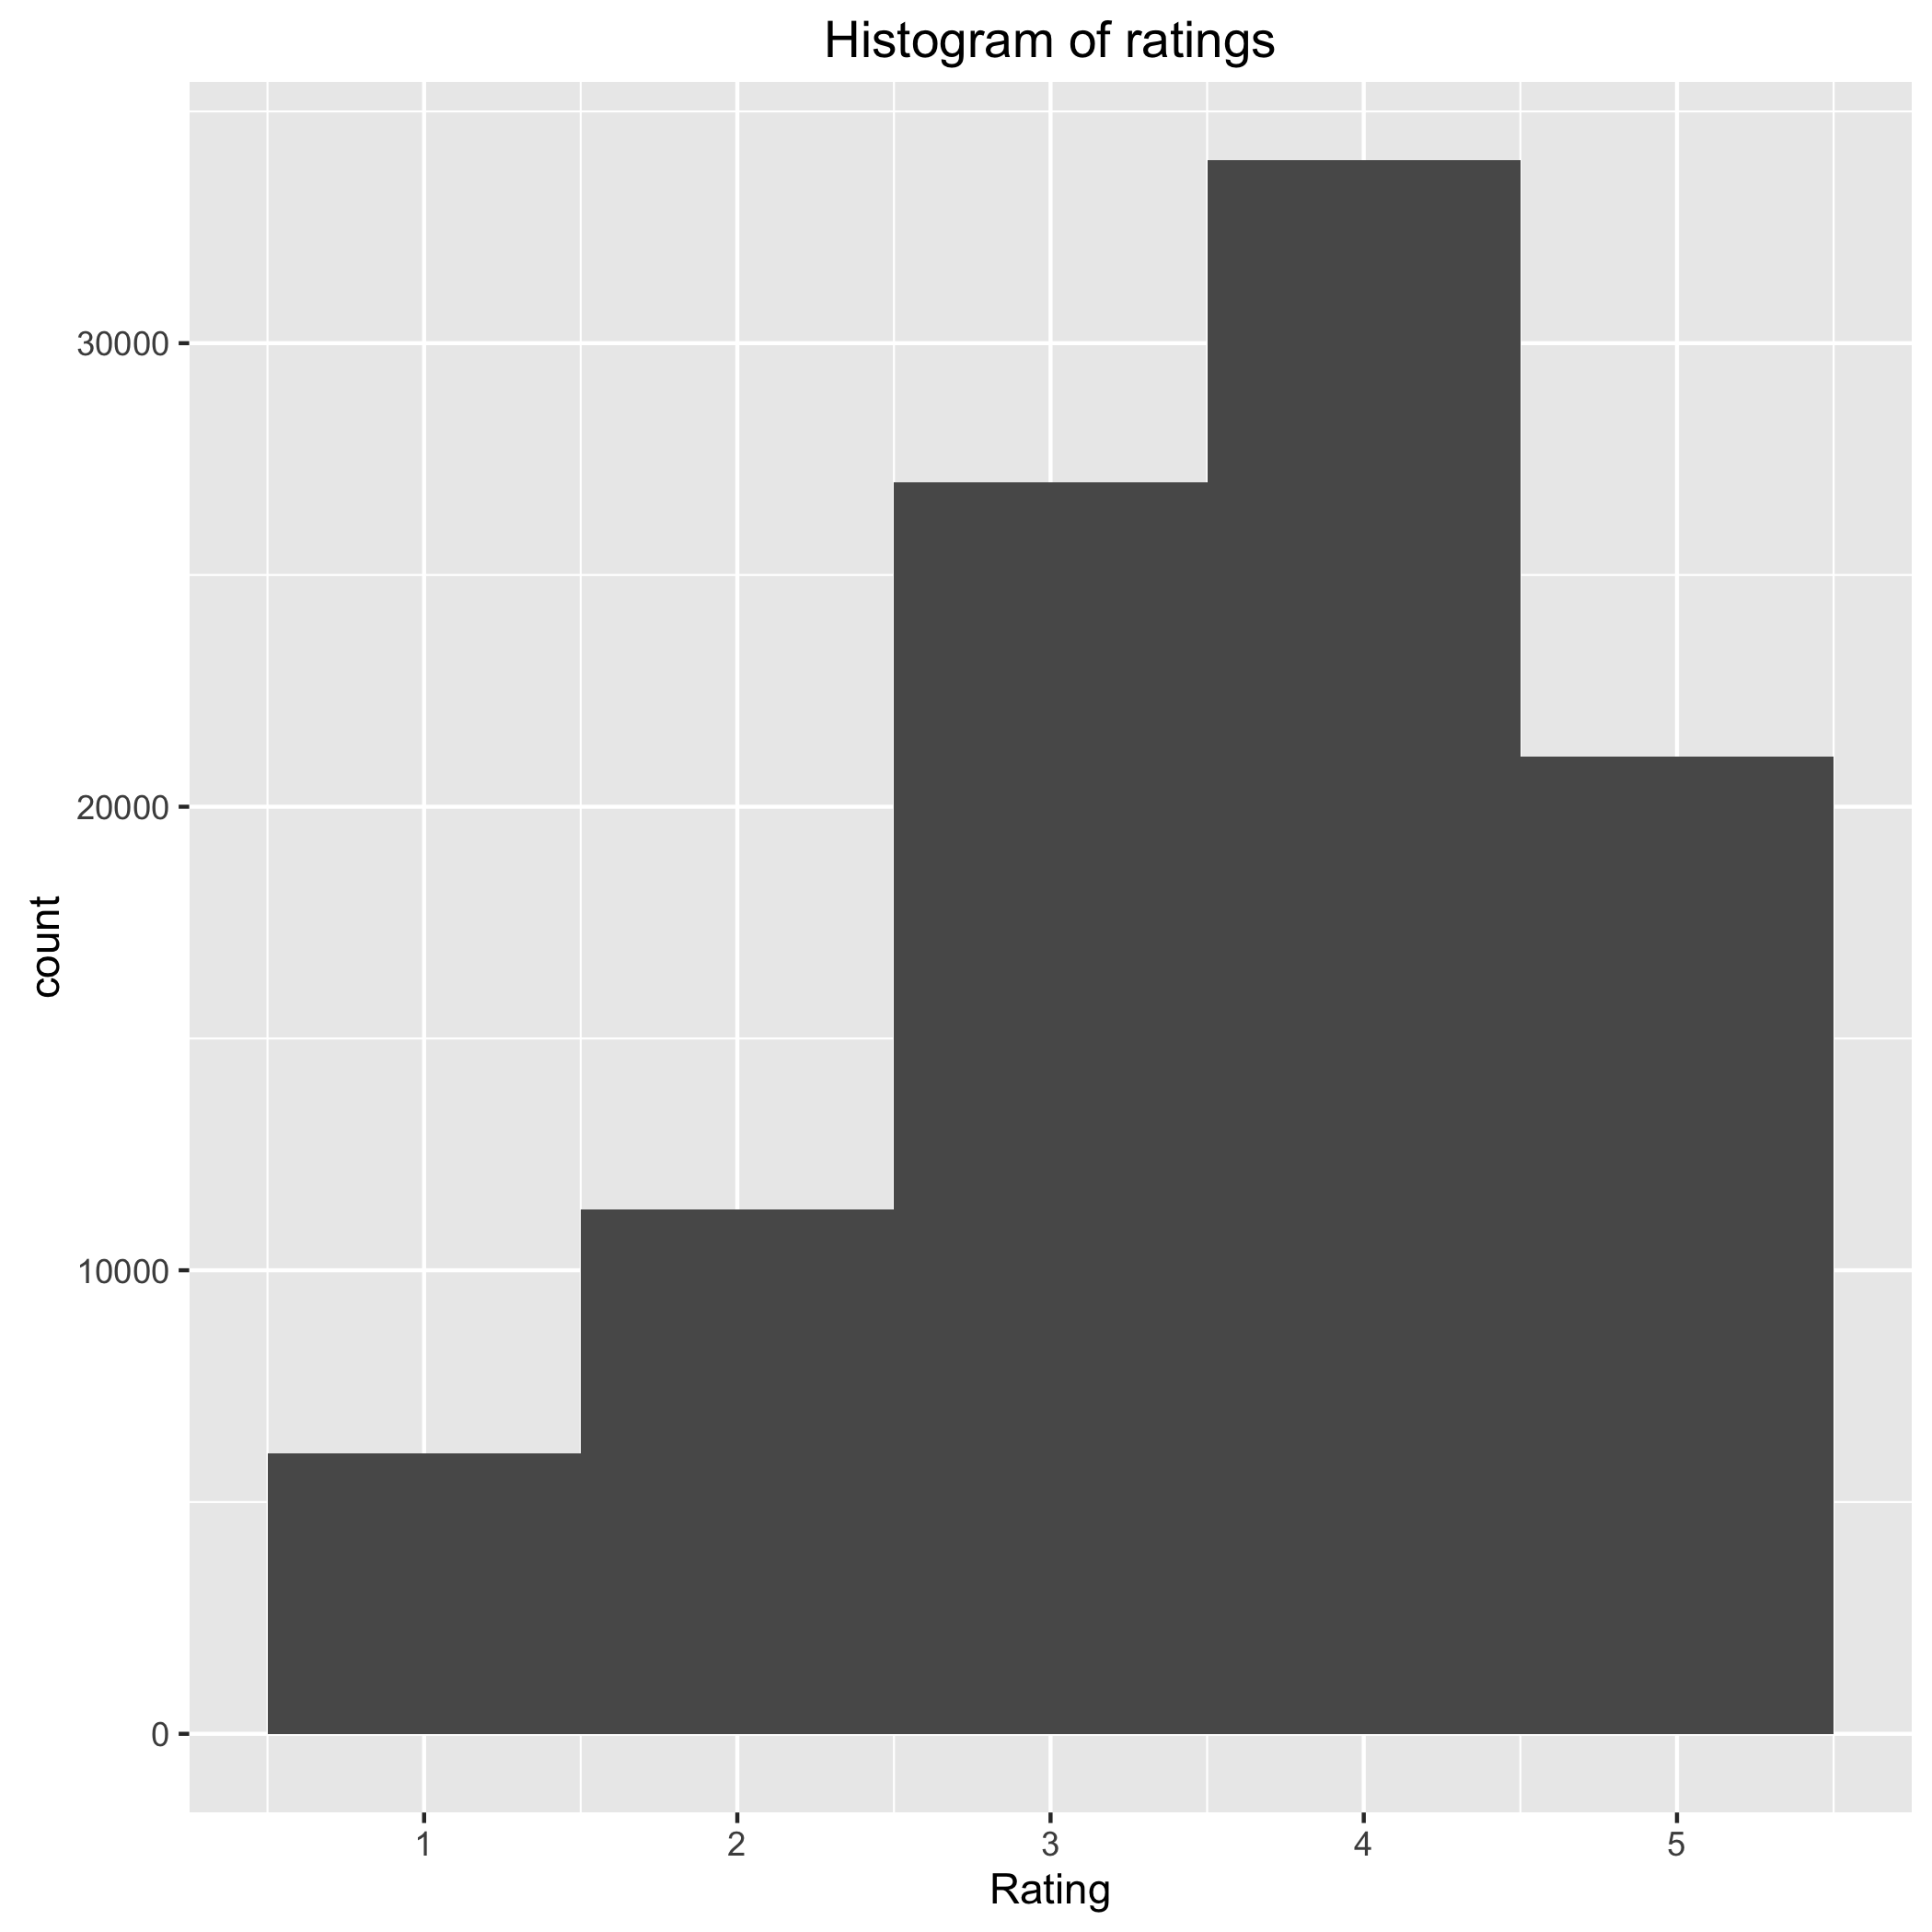
\includegraphics[width=2.8in]{rating.png}
	\caption{Rating Distribution}
	\label{fig:side:a}
\end{figure}

\begin{figure}
	\centering
	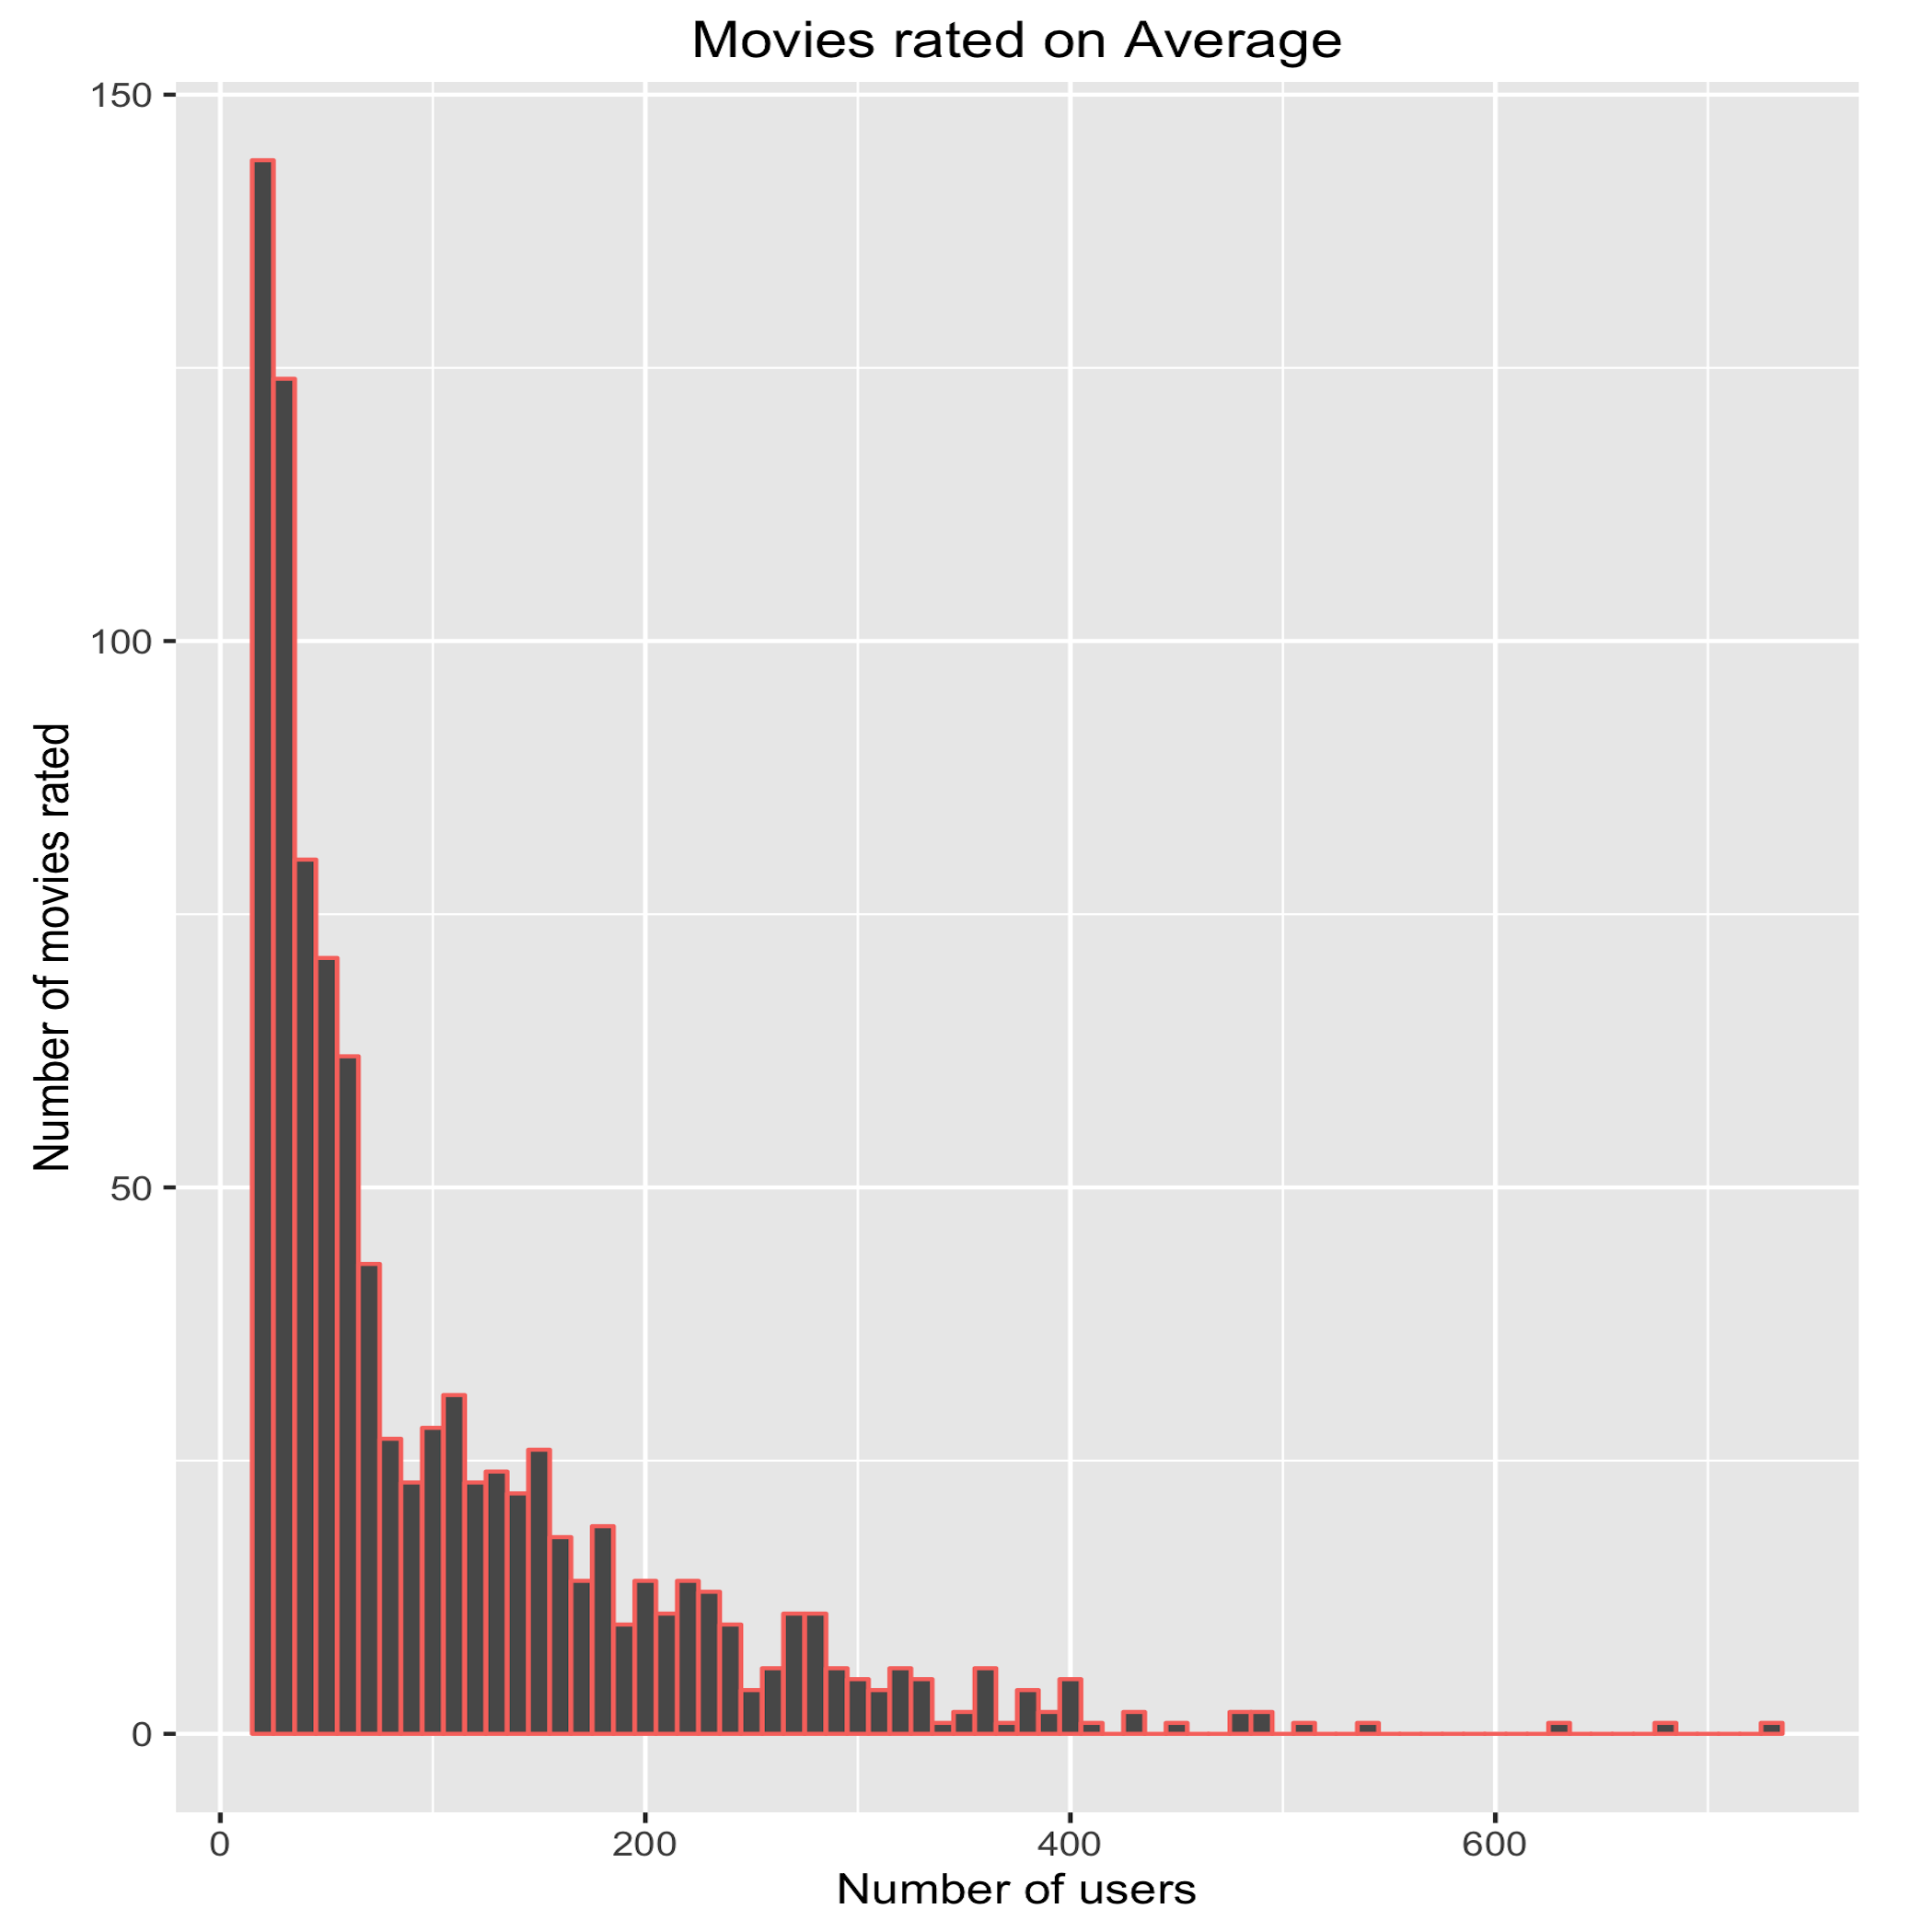
\includegraphics[width=2.8in]{user_rating.png}
	\caption{User Rating Count Distribution}
	\label{fig:side:a}
\end{figure}

\begin{figure}
	\centering
	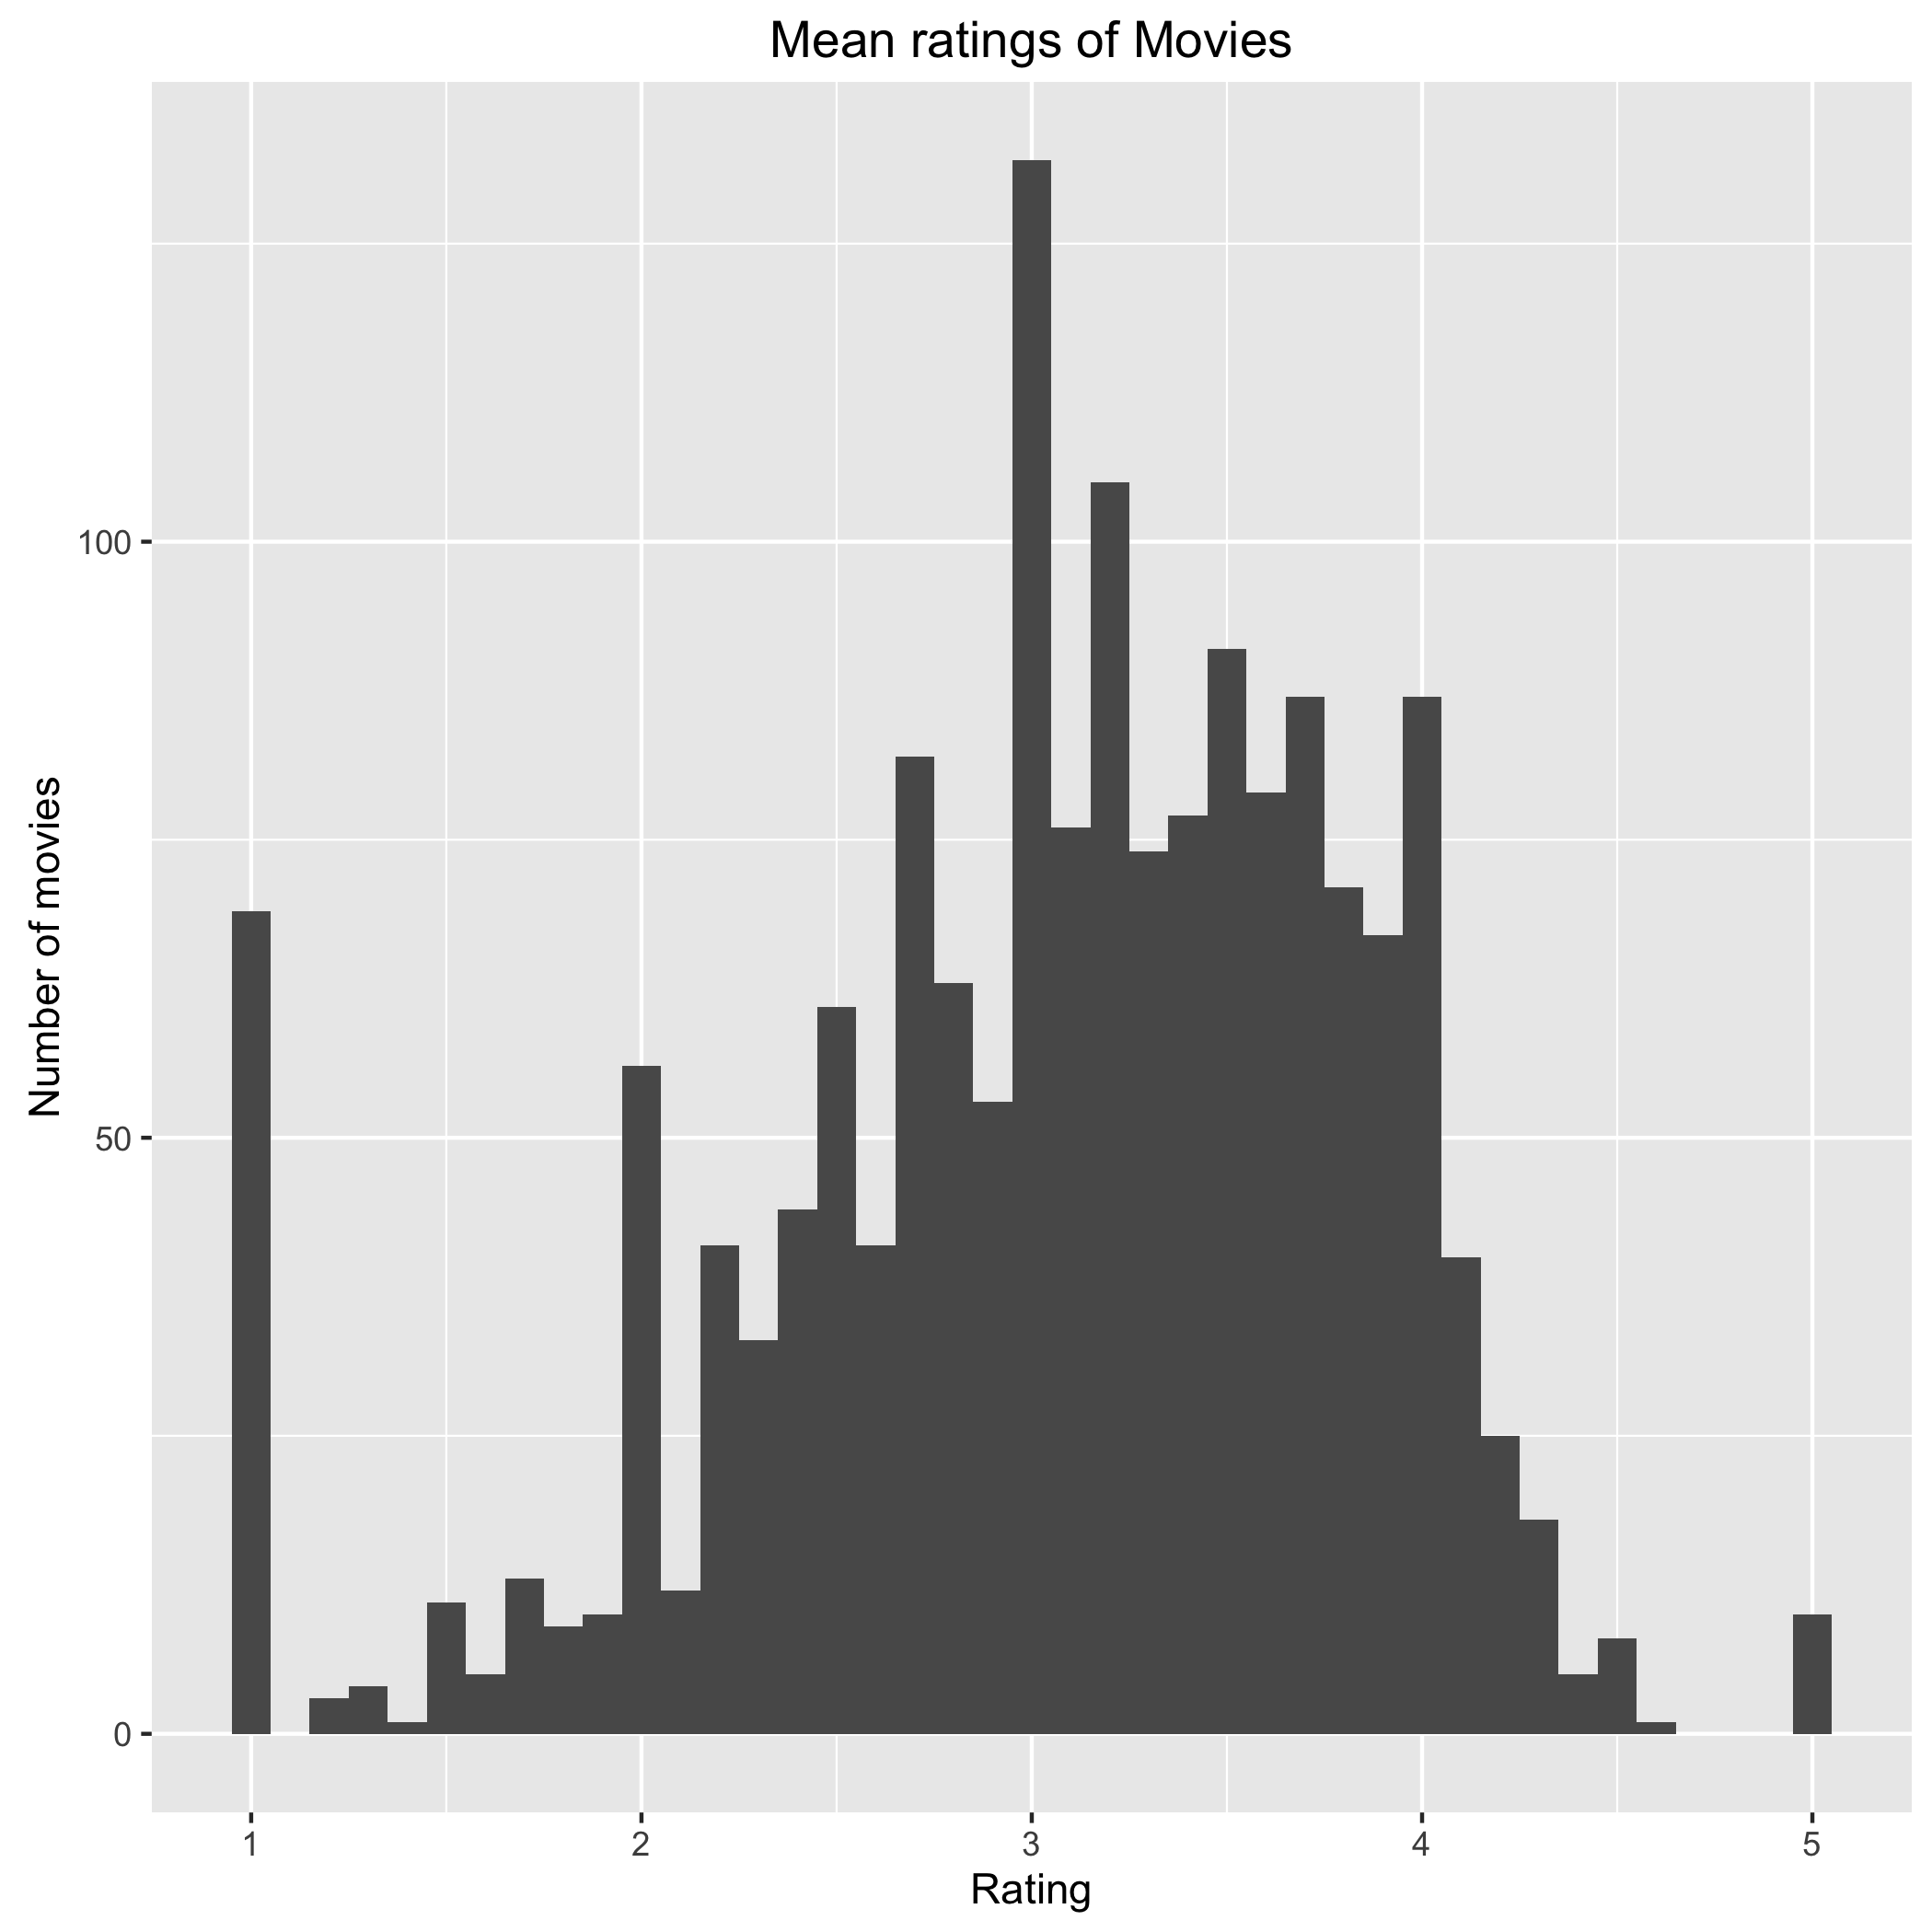
\includegraphics[width=2.8in]{movie_rating.png}
	\caption{Movie Average Rating Distribution}
	\label{fig:side:a}
\end{figure}

\subsubsection{Collaborative Filtering Results}
We apply both user-based CF and item-based CF for rating predicting. Also, we use a random prediction as a baseline. 

Figure 10 compares the prediction accuracy of the three methods. The  error rate shows that use-based CF works best among these three methods with a RMSE error of less than 1. Item-based CF is not as good as use-based CF. Its RMSE error rate is slightly higher than user-based CF. One possible reason about this difference is when and how we generating recommendations. User-based CF saves the whole matrix and then generates the recommendation at predict by finding the closest user. While item-based CF saves only k closest items in the matrix and doesn’t have to save everything. It is pre-calculated and predict simply reads off the closest items. We can see that the MAE of user-based CF and item-based CF are nearly the same. MAE is always smaller than RMSE because RMSE will enlarge the penalty on incorrect predictings. It is not surprise that Random approach is the worst because it only set a random rating between 1 to 5 for each movie by users.

\begin{figure}
	\centering
	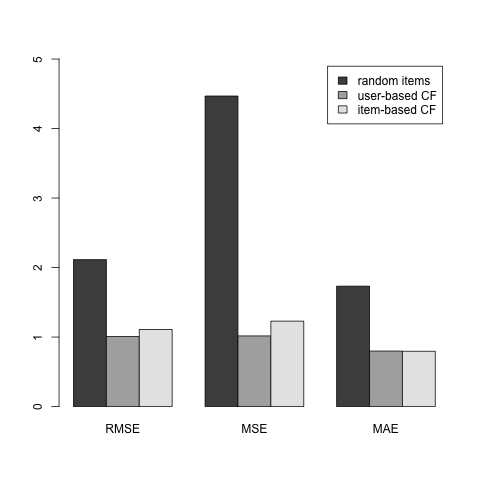
\includegraphics[width=2.8in]{RMSE.png}
	\caption{RMSE}
	\label{fig:side:a}
\end{figure}

We compared the performance of Random, user-based CF and item-based CF by changing the parameter n. That is we evaluate top-1, top-3, top-5, top-10, top-15 and top-20 recommendation lists. We can visualize the results by ploting ROC curves(Figure 11) and precision-recall curves (Figure12). 

ROC curve is a plot of the true positive rate against the false positive rate for the different possible cutpoints of a diagnostic test. The area under the curve is a measure of the accuracy. Thus the closer the curve follows the left-hand border and then the top border of the ROC space, the more accurate the test. The ROC curves show the same result with the former part. We can see that under a varying range of top-N list, the performance of user-based CF is always the best following by item-based CF. Random method is the worst. Besides, with the increasing of n, the differences of the TPR against FPR among the three becoming larger.

Different form ROC whose goal is to be in the upper-left-hand corner, the goal of precision-recall space is to be in the upper-right-hand corner, and the PR curves in Figure 11 show that there user-based CF works quite well while item-based CF still has vast room for improvement.

\begin{figure}
	\centering
	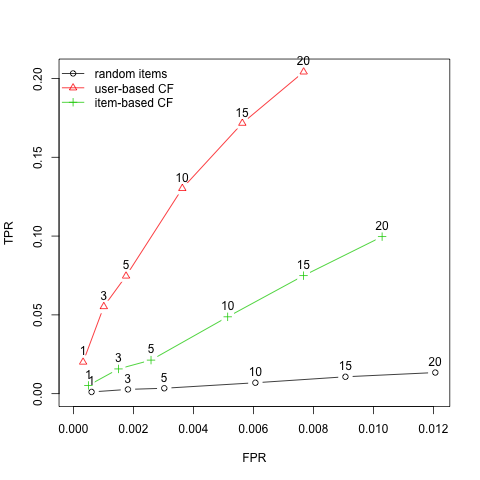
\includegraphics[width=2.8in]{ROC.png}
	\caption{ROC Curves}
	\label{fig:side:a}
\end{figure}

\begin{figure}
	\centering
	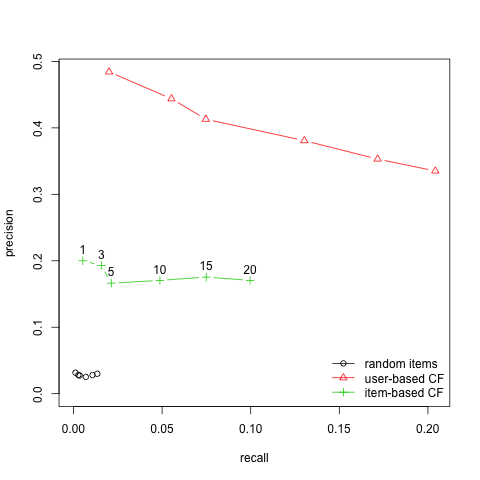
\includegraphics[width=2.8in]{precision_recall.png}
	\caption{Precision and Recall Curves}
	\label{fig:side:a}
\end{figure}

We also meatured the prediction time of each method. Table 4 shows the model time and prediction time of each applied algorithms. 
\begin{table}
	\caption{Running time of three algorithms}
	\begin{center}
		\begin{tabular}{ccc}
			\hline
			\rule{0pt}{12pt}Method  & \rule{0pt}{12pt}model time   &\rule{0pt}{12pt} prediction time\\
			\hline\rule{0pt}{12pt}
			Random    &   0.025sec & \ 	0.062sec \\
			User-based  &   0.054sec & \ 	0.859sec\\
			Item-based  &   37.911sec & \      0.591sec\\
			\hline
		\end{tabular}
	\end{center}
\end{table}

Table 4 shows that Random approach is the fastest as it involves in little computation. Both user-based and item-based CF need to calculate similarities between users or items, which is a considerable computation. We noticed that item-based CF takes plenty of time on training model. This is because the number of ratings a movie receives is greater than the number of rating a user has rated. Therefore, computing similarity between items involving in larger data which apparently costs more time. 
% An example of a floating figure using the graphicx package.
% Note that \label must occur AFTER (or within) \caption.
% For figures, \caption should occur after the \includegraphics.
% Note that IEEEtran v1.7 and later has special internal code that
% is designed to preserve the operation of \label within \caption
% even when the captionsoff option is in effect. However, because
% of issues like this, it may be the safest practice to put all your
% \label just after \caption rather than within \caption{}.
%
% Reminder: the "draftcls" or "draftclsnofoot", not "draft", class
% option should be used if it is desired that the figures are to be
% displayed while in draft mode.
%
%\begin{figure}[!t]
%\centering
%\includegraphics[width=2.5in]{myfigure}
% where an .eps filename suffix will be assumed under latex, 
% and a .pdf suffix will be assumed for pdflatex; or what has been declared
% via \DeclareGraphicsExtensions.
%\caption{Simulation results for the network.}
%\label{fig_sim}
%\end{figure}

% Note that the IEEE typically puts floats only at the top, even when this
% results in a large percentage of a column being occupied by floats.


% An example of a double column floating figure using two subfigures.
% (The subfig.sty package must be loaded for this to work.)
% The subfigure \label commands are set within each subfloat command,
% and the \label for the overall figure must come after \caption.
% \hfil is used as a separator to get equal spacing.
% Watch out that the combined width of all the subfigures on a 
% line do not exceed the text width or a line break will occur.
%
%\begin{figure*}[!t]
%\centering
%\subfloat[Case I]{\includegraphics[width=2.5in]{box}%
%\label{fig_first_case}}
%\hfil
%\subfloat[Case II]{\includegraphics[width=2.5in]{box}%
%\label{fig_second_case}}
%\caption{Simulation results for the network.}
%\label{fig_sim}
%\end{figure*}
%
% Note that often IEEE papers with subfigures do not employ subfigure
% captions (using the optional argument to \subfloat[]), but instead will
% reference/describe all of them (a), (b), etc., within the main caption.
% Be aware that for subfig.sty to generate the (a), (b), etc., subfigure
% labels, the optional argument to \subfloat must be present. If a
% subcaption is not desired, just leave its contents blank,
% e.g., \subfloat[].


% An example of a floating table. Note that, for IEEE style tables, the
% \caption command should come BEFORE the table and, given that table
% captions serve much like titles, are usually capitalized except for words
% such as a, an, and, as, at, but, by, for, in, nor, of, on, or, the, to
% and up, which are usually not capitalized unless they are the first or
% last word of the caption. Table text will default to \footnotesize as
% the IEEE normally uses this smaller font for tables.
% The \label must come after \caption as always.
%
%\begin{table}[!t]
%% increase table row spacing, adjust to taste
%\renewcommand{\arraystretch}{1.3}
% if using array.sty, it might be a good idea to tweak the value of
% \extrarowheight as needed to properly center the text within the cells
%\caption{An Example of a Table}
%\label{table_example}
%\centering
%% Some packages, such as MDW tools, offer better commands for making tables
%% than the plain LaTeX2e tabular which is used here.
%\begin{tabular}{|c||c|}
%\hline
%One & Two\\
%\hline
%Three & Four\\
%\hline
%\end{tabular}
%\end{table}


% Note that the IEEE does not put floats in the very first column
% - or typically anywhere on the first page for that matter. Also,
% in-text middle ("here") positioning is typically not used, but it
% is allowed and encouraged for Computer Society conferences (but
% not Computer Society journals). Most IEEE journals/conferences use
% top floats exclusively. 
% Note that, LaTeX2e, unlike IEEE journals/conferences, places
% footnotes above bottom floats. This can be corrected via the
% \fnbelowfloat command of the stfloats package.




\section{Conclusion}
Knowledge discovery in database is one of the most important tasks in database systems. In this project, we aim to study different data mining algorithms and their applications. We use the IMDB data and Movielens data as our dataset, applying four main techniques of data mining- classifacation, clustering, association rules and rating prediction. We first tried to create a database in MySQL, a third part tool IMDBPY was applied to utilize our work, and we got 21 tables. For the convenience of exercising different mining techniques, we adopt R for analysis. We extract a sample from the IMDB database, applying three classification algorithms including K-NN, C4,5, and Naive Bayes, ROCK clustering and apriori algorithm. The compared results of classification shows that the Naive Bayes Classifier is the most suitable one for our dataset with an accuracy of 34\%. The other two classifiers-C4.5, K-NN did not perform well, with only 17\% and 5\% accuracy respectively. After applying ROCK clustering, the dataset is divided into 723 clusters which is much larger than the original 29 types of genres. We also tried to find the relationships between actors and crews as well as between crews and genre. We usesd apriori algorithms, listing 10 potential rules. Finally, we used collaborative filtering method for rating prediction on MovieLens dataset. We exercised both user-based CF and item-based CF, compared their performance regarding RMSE error. The results show that user-based CF works better than item-based CF in our data.






% conference papers do not normally have an appendix


% use section* for acknowledgment






% trigger a \newpage just before the given reference
% number - used to balance the columns on the last page
% adjust value as needed - may need to be readjusted if
% the document is modified later
%\IEEEtriggeratref{8}
% The "triggered" command can be changed if desired:
%\IEEEtriggercmd{\enlargethispage{-5in}}

% references section

% can use a bibliography generated by BibTeX as a .bbl file
% BibTeX documentation can be easily obtained at:
% http://mirror.ctan.org/biblio/bibtex/contrib/doc/
% The IEEEtran BibTeX style support page is at:
% http://www.michaelshell.org/tex/ieeetran/bibtex/
%\bibliographystyle{IEEEtran}
% argument is your BibTeX string definitions and bibliography database(s)
%\bibliography{IEEEabrv,../bib/paper}
%
% <OR> manually copy in the resultant .bbl file
% set second argument of \begin to the number of references
% (used to reserve space for the reference number labels box)
\begin{thebibliography}{10}
\bibitem{jiawei}
Jiawei Han, Micheline Kamber, Jian Pei. \emph{Data Mining Concepts and Techniques}, 3rd Edition, 2012.
\bibitem{Usama}
Usama Fayyad, Gregory Piatetsky-Shapiro, and Padhraic Smyth. \emph{From Data Mining to Knowledge Discovery in Databases}. AI Magazine Volume 17 Number 3, 1996.
\bibitem{fengchen}
Feng Chen, Pan Deng, Jianfu Wan and etc. \emph{Data Mning for the Internet of Things: Literature Review and cChallenges}. International Journal of Distributed Sensor Networks, 2015.
\bibitem{Bruno}
Bruno Pradel, Savaneary Sean,  Julien Delporte. \emph{A Case Study in a Recommender System Based on Purchase Data}. Proceedings of the 17th ACM SIGKDD international conference on Knowledge discovery and data mining, Pages 377-385, 2011.
\bibitem{Daniar}
Daniar Asanov. \emph{Algorithms and Methods in Recommender Systems.} Berlin Institute of Technology, Berlin, Germany, 2011.
\bibitem{imdb}
http://www.imdb.com/
\bibitem{movielens}
http://movielens.umn.edu/ 
\bibitem{imdbpy}
http://imdbpy.sourceforge.net/
\bibitem{Michael}
Michael Hahsler \emph{A Probabilistic Comparison of Commonly Used Interest Measures for Association Rules.} 2015.
\bibitem{Everitt}
Everitt, B. S., Landau, S., Leese, M. and Stahl, D. \emph{Miscellaneous Clustering Methods, in Cluster Analysis, 5th Edition.} John Wiley \& Sons, Ltd, Chichester, UK, 2011.
 \bibitem{Narasimha}
 Narasimha Murty, M., Susheela Devi, V. \emph{Pattern Recognition: An Algorithmic Approach.} 2011.
 \bibitem{Quinlan}
 Quinlan, J. R. \emph{ Induction of Decision Trees. Mach. Learn. } 1986.
 \bibitem{Guha}
 Guha S, Rastogi R, Shim K. \emph{ROCK: A robust clustering algorithm for categorical attributes.} Data Engineering, 15th International Conference on. IEEE, 1999: 512-521.
\bibitem{survey}
Xiaoyuan Su, Taghi M. Khoshgoftaar. \emph{A Survey of Collaborative Filtering Techniques.}
Advances in Artificial Intelligence (2009) 421425.
\bibitem{Herlocker}
Herlocker, J. L., J. A. Konstan, L. G. Terveen, and J. T. Riedl. Evaluating Collaborative
Filtering Recommender Systems. ACM Transactions on Information Systems, 22(1):5-53,
2004. 
\bibitem{Borgelt}
Borgelt C, Kruse R. \emph{Induction of association rules: Apriori implementation} Compstat. Physica-Verlag HD, 2002: 395-400.

\end{thebibliography}




% that's all folks
\end{document}


